\documentclass[12pt,a4paper]{report}
\usepackage[utf8]{inputenc}

\usepackage[T1]{fontenc} %to search pdf
\usepackage{ucs}
\usepackage{amsmath, amssymb}
\usepackage{amsfonts}
\usepackage{amssymb}
\usepackage[brazil]{babel} % Comentário, Português do Brasil
\usepackage{graphicx}
\usepackage{setspace}
\usepackage{fancyhdr}
\usepackage[pdftex, colorlinks,linkcolor=black,hyperindex]{hyperref}
\usepackage{wrapfig}
\usepackage{wallpaper}
\usepackage{subfig}
\usepackage{float}
\usepackage{esvect}


\hypersetup{
    colorlinks,
    citecolor=black,
    filecolor=black,
    linkcolor=black,
    urlcolor=blue
}

\graphicspath{{../user_guide_figures/}{../user_guide_figures/invesalius_screen/}{../user_guide_figures/icons/}}

\author{Centro de Tecnologia da Informação Renato Archer}
\title{Software InVesalius - Manual de Usuário}
\date{}

\begin{document}

\thispagestyle{empty}

\begin{flushright}

\flushright \scalebox{2.5}{\sffamily{\textbf{InVesalius}}}
\par
\vspace{180pt}
\scalebox{2.8}{\sffamily User Guide}
\ThisLLCornerWallPaper{1}{capa2.png}

\begin{figure}[h!]
\flushright 

\includegraphics[scale=0.5, bb = 0 0 300 601]{logo_cti.jpg}
\end{figure}		

\end{flushright}
\newpage
\vspace*{10pt}
\thispagestyle{empty}

\begin{center} \emph{\begin{large}  About InVesalius \end{large}}
\vspace{2pt}
\end{center}

\onehalfspacing
 		
%InVesalius é um software público para a área de saúde que realiza análise e segmentação de
%modelos anatômicos virtuais, possibilitando a confecção de modelos físicos com o auxílio da
%prototipagem rápida.
%A partir de imagens em duas dimensões (2D) obtidas por meio de equipamentos de Tomografia
%Computadorizada (TC) ou Ressonância Magnética (RM), o programa permite criar modelos
%virtuais em três dimensões (3D) correspondentes às estruturas anatômicas dos pacientes em
%acompanhamento médico.

InVesalius is a public health software that performs analysis and segmentation of
Virtual anatomical models, enabling the creation of physical models with the aid of
rapid prototyping (3D printing).
From two-dimensional (2D) images obtained by means of Tomography Computerized (CT) or Magnetic Resonance (MRI), the program allows to create
three-dimensional (3D) anatomical structures corresponding the patients in medical follow-up.

%O nome InVesalius é uma homenagem ao médico belga Andreas Vesalius (1514-1564),
%considerado o "pai da anatomia moderna".
%O software InVesalius é desenvolvido pelo CTI (Centro de Tecnologia da Informação Renato
%Archer), unidade do Ministério da Ciência e Tecnologia (MCT), desde 2001. Inicialmente, apenas
%o programa de instalação era distribuído gratuitamente. A partir de novembro de 2007,
%o InVesalius foi disponibilizado como software livre no Portal do Software Público
%(\href{http://www.softwarepublico.gov.br}{www.softwarepublico.gov.br}), consolidando comunidades de usuários e de desenvolvedores.
%Trata-se de uma ferramenta simples, livre e gratuita,
%robusta, multiplataforma, com comandos em Português, com funções claras e diretas, de fácil
%manuseio e rápida quando executada em microcomputador PC.

InVesalius name is a tribute to the Belgian doctor Andreas Vesalius (1514-1564),
considered the "father of modern anatomy".
InVesalius software is developed by CTI (Center for Information Technology Center Renato
Archer), a unit of the Brazilian Ministry of Science and Technology (MCT), since 2001. Initially, only
the installation program was distributed as freeware. On the November 2007
InVesalius was made available as free software and open source in the Public Software Portal
(\href{http://www.softwarepublico.gov.br}{www.softwarepublico.gov.br}), consolidating communities of users and developers.
It is a simple, easy to use, robust, cross-platform and free tool.

%O uso das tecnologias de visualização e análise tridimensional de imagens médicas, integradas
%ou não a prototipagem rápida, auxiliam o cirurgião no diagnóstico de patologias e permitem que
%seja realizado um planejamento cirúrgico detalhado, simulando com antecedência intervenções
%complexas, que podem envolver, por exemplo, alto grau de deformidade facial ou a colocação
%de próteses.

The use of visualization technologies and three-dimensional analysis of medical images , perhaps integrated with rapid prototyping, assists the surgeon in diagnosing pathologies and a detailed surgical planning, simulating complex interventions in advance, which may involve, for example, a high degree of facial deformity or of prosthetics.

%O InVesalius tem demonstrado grande versatilidade e vem contribuindo com diversas áreas,
%dentre as quais medicina, odontologia, veterinária, arqueologia e engenharia.

InVesalius has demonstrated great versatility and has contributed to several areas,
including medicine, dentistry, veterinary medicine, archeology and engineering.
		
\noindent

\tableofcontents
\chapter{Introdução}
Este manual tem como objetivo mostrar o uso das ferramentas
do InVesalius e também apresentar alguns conceitos para facilitar
a utilização do software.

O InVesalius é um software para auxiliar o profissional
de saúde no diagnóstico	e no planejamento cirúrgico. Cabe
ressaltar, porém, que todo software no contexto de diagnóstico é
totalmente suplementar, pois todo e qualquer ato cometido é de
inteira responsabilidade do profissional de saúde.

Além da medicina, é possível utilizar o software em outras áreas, como
arqueologia, veterinária, ou mesmo em aplicações industriais.
Como requisito básico, basta que as imagens a serem analisadas
estejam no padrão DICOM (\textsl{Digital Imaging Communications in Medicine}).
Até o presente momento, o InVesalius reconstrói
imagens provindas de tomógrafos e de aparelhos de ressonância magnética.
Para operar o software, basta ter conhecimentos básicos de 
informática. Noções básicas sobre imagens médicas podem contribuir para o
melhor entendimento das operações.


\section{Conceitos importantes}
Nesta seção, discutiremos alguns conceitos necessários para melhor
entendimento e operação do software.


\subsection{DICOM (\textit{Digital Image Communications in Medicine})}			
DICOM é um padrão relativo à transmissão, ao armazenamento e
ao tratamento de imagens médicas. O padrão prevê diversas modalidades de imagens médicas,
como imagens provindas de equipamentos de tomografia computadorizada, ressonância magnética,
ultrassom, eletrocardiograma, entre outras.

Uma imagem DICOM é composta por 2 itens principais, uma matriz contendo os pixels da
imagem e um conjunto de meta-informações. Essas informações contêm, por exemplo, o nome
do paciente, a modalidade da imagem e a posição da imagem em relação ao espaço (no caso
de tomografia e ressonância).


\subsection{Tomografia Computadorizada - Médica}
A tomografia computadorizada indica a radiodensidade dos tecidos, isto é, a média de
absorção de raios-X pelos tecidos. A radiodensiade é traduzida para a imagem em níveis
de cinza em uma escala chamada \textit{Hounsfield}, nome dado em homenagem a Godfrey
Newbold Hounsfield, um dos criadores da primeira máquina de tomografia computadorizada.

%\begin{wrapfigure}{c}{0.5\textwidth}
%  \begin{center}
%    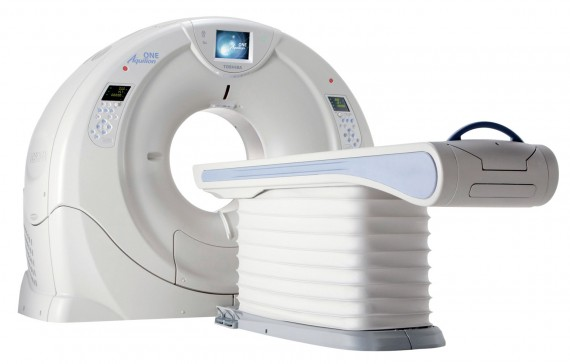
\includegraphics[scale=0.3]{img/tomografo.jpg}
%  \end{center}
%  \caption{Tomógrafo Médico http://www.toshibamedical.com.br}
%\end{wrapfigure}
\begin{figure}[!htb]
\centering
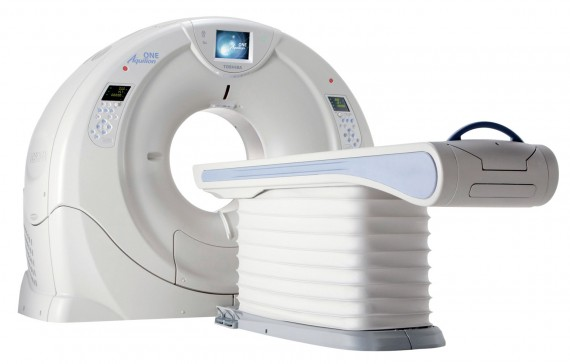
\includegraphics[scale=0.4]{img/tomografo.jpg}
\caption{Tomógrafo médico - www.toshibamedical.com.br}
\end{figure}

%\begin{figure}[!htb]
%\centering
%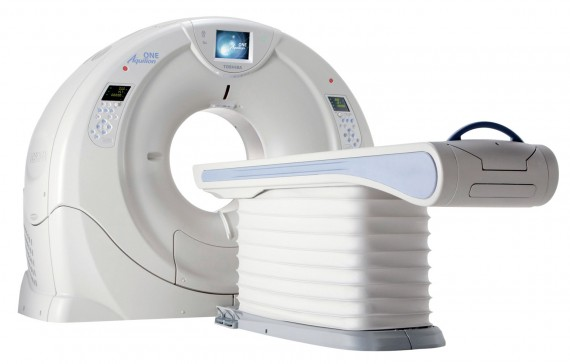
\includegraphics[scale=0.3]{img/tomografo.jpg}
%\caption{Tomógrafo Médico}
%\end{figure}

Nos aparelhos mais modernos, com um emissor de radiação e um banco de
sensores (também chamados de canais, variando de 2 até 256), que circundam o paciente
enquanto a maca é movimentada, formando uma espiral, é possível gerar uma
grande quantidade de imagens, simultaneamente, com pouca emissão de raios-X.


\subsubsection{Escala de Hounsfield}
Como citado na seção anterior, as imagens de tomografia computadorizada
são geradas em níveis de cinza, os quais são depois traduzidos na escala
de Hounsfield (HU). Os tons mais claros representam tecidos mais densos, e
os mais escuros, tecidos menos densos, como a pele e o cérebro.
A tabela \ref{tab:escala_hounsfield} apresenta alguns materiais e seus 
respectivos valores em HU (\textit{Hounsfield Unit}).


\begin{table}[h]
\centering
\caption{Escala de Hounsfield}
\begin{tabular}{lcc}\\
\hline % este comando coloca uma linha na tabela
Material & HU\\
\hline
\hline
Ar & -1000 ou menos\\
Gordura & -120\\
Água & 0\\
Músculo & 40\\
Contraste & 130\\
Osso & 400 ou mais\\
\hline
\end{tabular}
\label{tab:escala_hounsfield}
\end{table}


\subsection{Tomografia Computadorizada - Odontológica}

A tomografia computadorizada odontológica comumente trabalha com menos emissão
de radiação se comparada à tomografia computadorizada médica e, em consequência,
torna possível visualizar mais detalhes de regiões delicadas, como a cortical alveolar.

\begin{figure}[!htb]
\centering
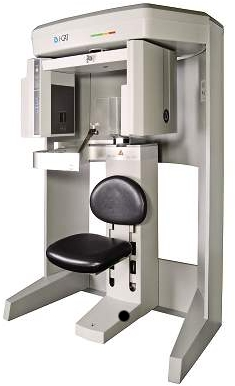
\includegraphics[scale=0.4]{img/feixe_conico.jpg}
\caption{Tomógrafo odontológico - www.kavo.com.br}
\end{figure}

A aquisição das imagens é feita com o paciente na vertical (ao contrário da tomografia médica,
em que o paciente fica na horizontal). Um emissor e um sensor de raios-X circundam o crânio
do paciente, formando um arco de $180^\circ$ ou $360^\circ$. As imagens geradas pelo tomógrafo
podem ser interpretadas como um volume com o crânio do paciente imerso. Esse volume é "fatiado"
pelo software do aparelho, podendo-se gerar imagens com espaçamentos diferentes ou outros
tipos de imagens, como a visão panorâmica da região de interesse.

As imagens adquiridas por tomógrafos odontológicos costumam exigir um maior pós-processamento
quando é necessário separar (segmentar) determinadas estruturas usando outros softwares como
o InVesalius. Isso ocorre porque, normalmente, essas imagens possuem mais níveis de cinza que
a escala de Hounsfield, o que torna o uso de padrões de segmentação \textit{(presets)} menos
eficiente. Outra característica bastante comum nas imagens provindas de tomógrafos
odontológicos é a alta presença de ruídos do tipo \textit{speckle} e a presença de outros
ruídos normalmente causados por uso de próteses de amálgama pelo paciente.


\subsection{Ressonância Magnética}

A ressonância magnética é um exame realizado sem o uso de radiação ionizante. Em vez disso,
é utilizado um forte campo magnético para alinhar os átomos de algum elemento presente em
nosso corpo, comumente o hidrogênio. Após o alinhamento, são disparadas ondas de rádio, e os
átomos são excitados. Os sensores medem o tempo que os átomos de hidrogênio demoram para se
alinhar novamente. Com isso, é possível determinar qual é o tipo de tecido, pois tecidos
diferentes apresentam quantidades diferentes de átomos de hidrogênio.

Para evitar interferências e melhorar a qualidade do sinal de radiofrequência, além de o
paciente ficar dentro do equipamento, é colocada uma bobina na região de interesse.

 
\begin{figure}[!htb]
\centering
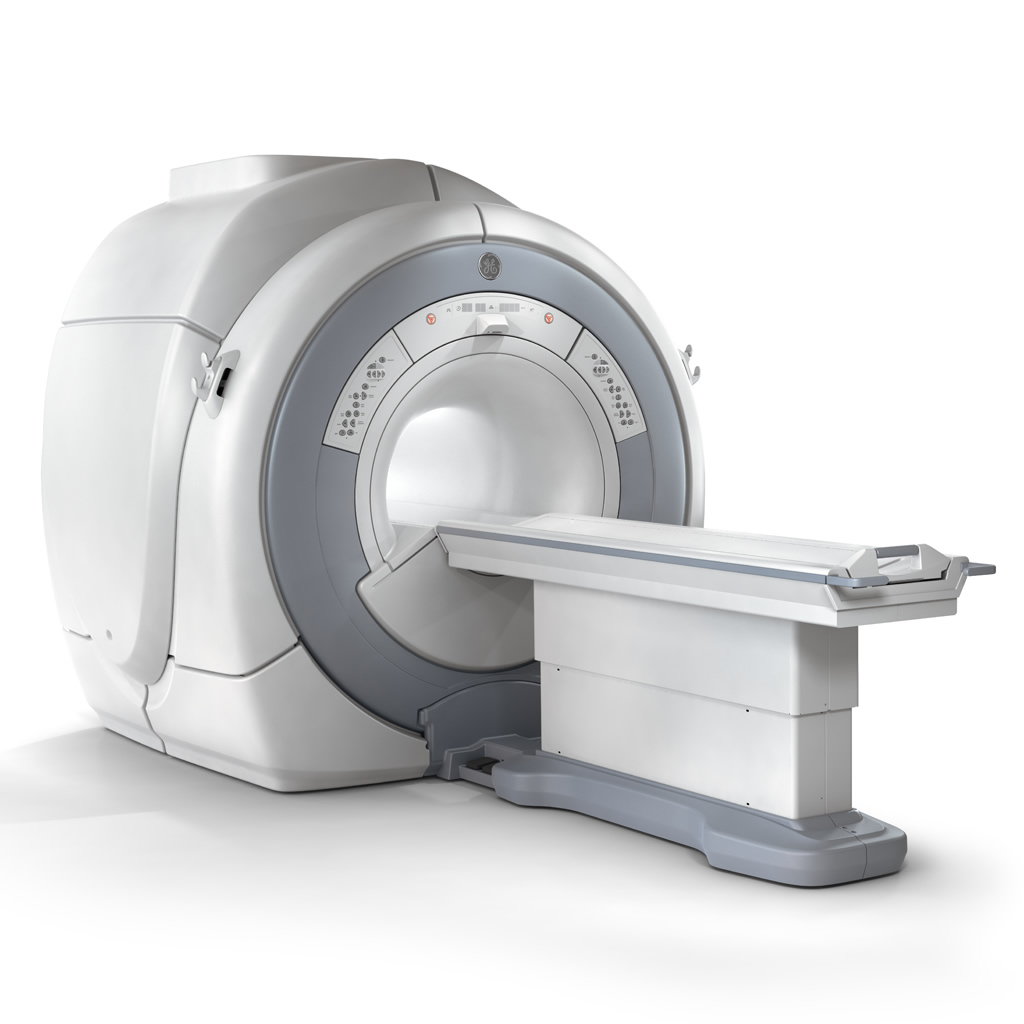
\includegraphics[scale=0.2]{img/rm_ge.jpg}
\caption{Equipamento de ressonância magnética - www.gehealthcare.com}
\end{figure}

\begin{figure}[!htb]
\centering
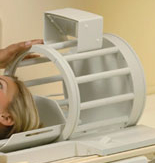
\includegraphics[scale=0.8]{img/bobina.jpg}
\caption{Bobina - www.healthcare.philips.com}
\end{figure}


\section{Recursos necessários}
O InVesalius é projetado para executar em computadores pessoais, como
\textit{desktops} e \textit{notebooks}. Atualmente, ele é compatível com
os seguintes sistemas operacionais:\\
- MS-Windows (XP, Vista, Windows 7)\\
- GNU/Linux (Ubuntu, Mandriva, Fedora)\\
- Apple Mac OS X

O desempenho do InVesalius depende, principalmente, da quantidade de fatias
reconstruídas (imagens abertas pelo software), da quantidade de memória RAM
disponível, da frequência do processador e da arquitetura do sistema operacional
(32 \textit{bits} ou 64 \textit{bits}).

Vale ressaltar, como regra geral, que quanto maior a quantidade de memória RAM
disponível no sistema, maior será o número de fatias que podem ser abertas
simultaneamente para um dado estudo. Por exemplo, com 1 GB de memória disponível,
pode-se abrir cerca de 300 fatias com resolução de 512x512 \textit{pixels}.
Já com 4 GB de memória, pode-se abrir em torno de 1000 imagens com a mesma
resolução.

			
\subsection{Configurações mínimas}
Sistema Operacional de 32 \textit{bits}\\
Processador Intel Pentium 4 ou equivalente, com frequência de 1,5 GHz\\
1 GB de memória RAM\\
80 GB de disco rígido\\
Placa gráfica com 64 MB de memória\\
Resolução de vídeo de 1024x768 \textit{pixels}


\subsection{Configurações recomendadas}
Sistema Operacional de 64 \textit{bits}\\
Processador Intel Core 2 Duo ou equivalente, com frequência de 2,5 GHz\\
4 GB de memória RAM\\
180 GB de disco rígido\\
Placa gráfica NVidia ou ATI, com 128 MB de memória\\
Resolução de vídeo de 1024x768 \textit{pixels}


\chapter{Instalação}

\section{MS-Windows}

Para instalar o InVesalius no MS-Windows, basta executar o programa instalador.
Quando aparecer uma janela pedindo para confirmar a execução do arquivo, clique
em \textbf{Sim}.

\begin{figure}[!htb]
\centering
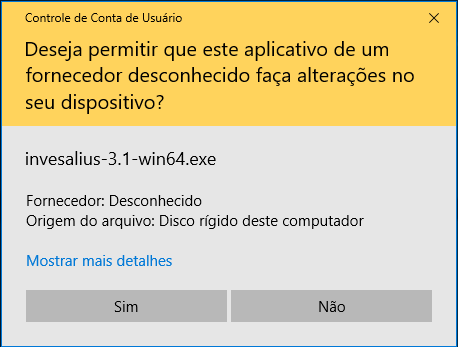
\includegraphics[scale=0.5]{installation_exec_pt.png}
\end{figure}

\newpage
Uma nova janela pedirá para selecionar o idioma do instalador. Selecione
o idioma e clique em \textbf{OK}.

\begin{figure}[!htb]
\centering
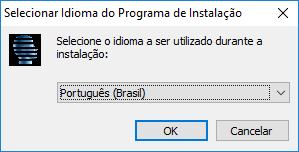
\includegraphics[scale=0.7]{installation_select_language_pt.png}
\end{figure}
 
\hspace{.2cm}

Em seguida, será exibida a janela do instalador. Clique em \textbf{Avançar}.

\begin{figure}[!htb]
\centering
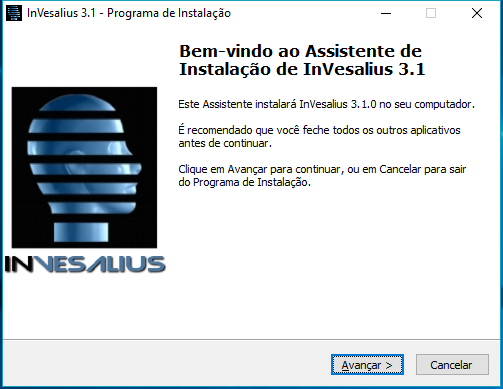
\includegraphics[scale=0.7]{installation_welcome_pt.png}
\end{figure}

\newpage

Selecione \textbf{Eu aceito os termos do Contrato} e clique em \textbf{Avançar}.

\begin{figure}[!htb] 
\centering
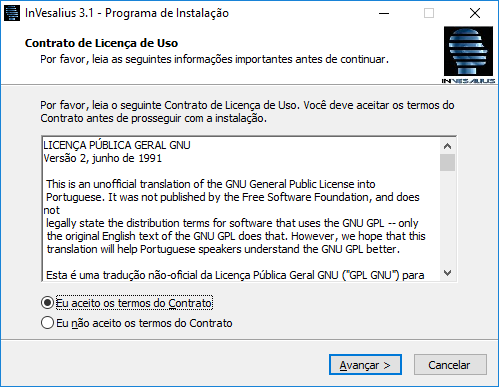
\includegraphics[scale=0.7]{installation_license_pt.png}
\end{figure}

\hspace{.2cm}

Clique em \textbf{Avançar} novamente. 

\begin{figure}[!htb]  
\centering
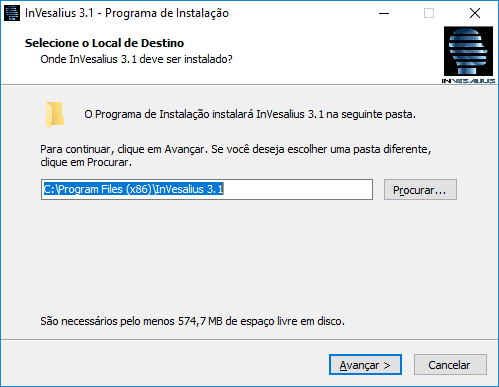
\includegraphics[scale=0.7]{installation_folder_pt.png}
\end{figure}

\newpage

Clique em \textbf{Avançar}.
\begin{figure}[!htb]
\centering
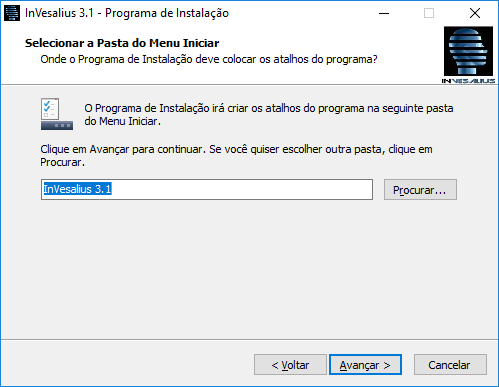
\includegraphics[scale=0.7]{installation_program_name_pt.png}
\end{figure}

\hspace{.2cm}

Selecione \textbf{Criar um ícone na Área de Trabalho} e clique em \textbf{Avançar}.

\begin{figure}[!htb]
\centering
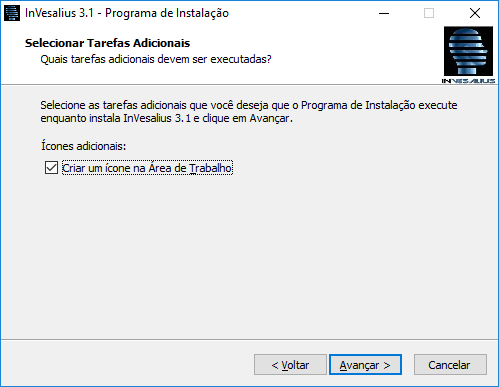
\includegraphics[scale=0.7]{installation_desktop_shortcut_pt.png}
\end{figure}

\newpage

Clique em \textbf{Instalar}.

\begin{figure}[!htb]
\centering
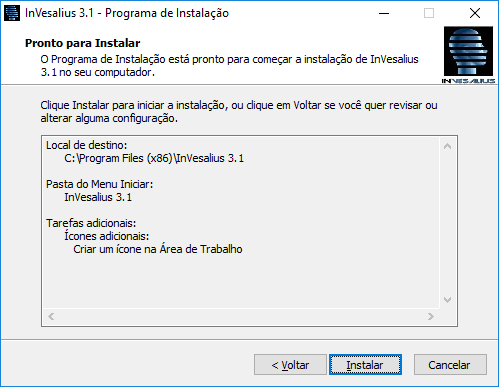
\includegraphics[scale=0.7]{installation_resume_pt.png}
\end{figure}

\hspace{.2cm}

Enquanto o software é instalado, será exibida uma janela com o progresso
da instalação.

\begin{figure}[!htb]
\centering
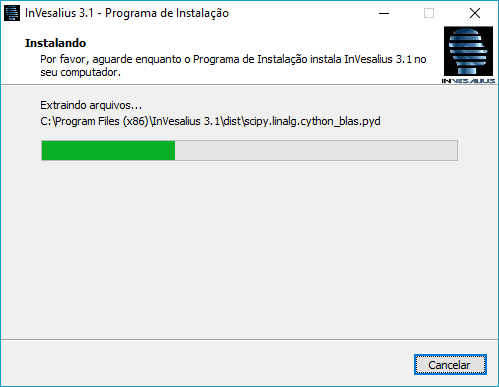
\includegraphics[scale=0.7]{installation_progress_pt.png}
\end{figure}

\newpage

Para executar o InVesalius após a instalação, clique em \textbf{Concluir}.

\begin{figure}[!htb]
\centering
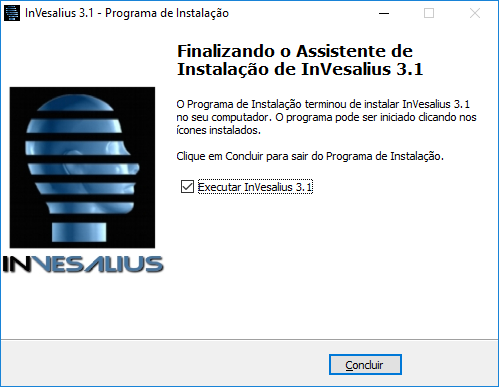
\includegraphics[scale=0.7]{installation_finish_pt.png}
\end{figure}

\hspace{.2cm}

Caso seja a primeira vez em que o software é instalado, será exibida uma janela
para selecionar o idioma do InVesalius. Selecione o idioma desejado e clique em
\textbf{OK}.

\begin{figure}[!htb]
\centering
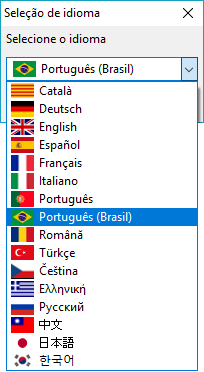
\includegraphics[scale=0.7]{invesalius_language_select_pt.png}
\end{figure}

\newpage

Enquanto o InVesalius é carregado, é exibida uma janela de abertura como a da figura
seguinte.

\begin{figure}[!htb]
\centering
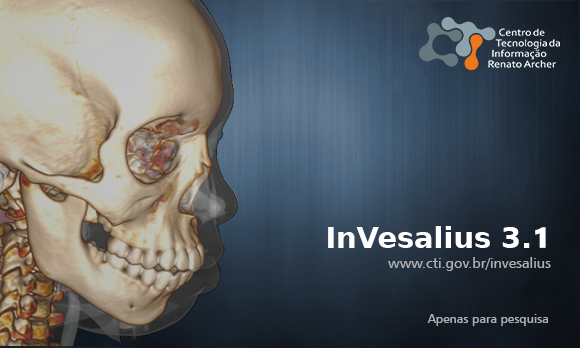
\includegraphics[scale=0.4]{splash_pt.png}
\end{figure}

\hspace{.2cm}

Em seguida, a janela principal do programa é aberta.

\begin{figure}[!htb]
\centering
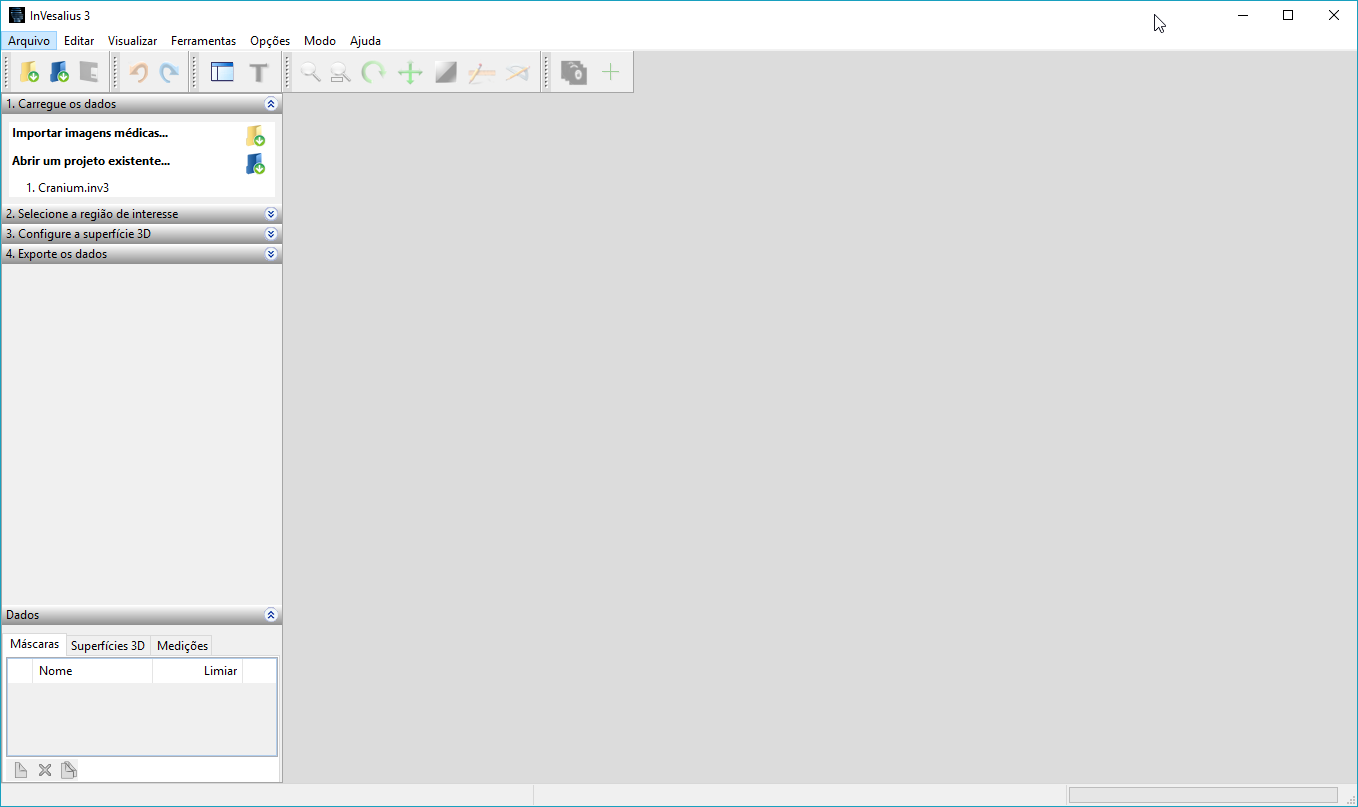
\includegraphics[scale=0.4]{main_window_without_project_pt.png}
\end{figure}

\section{Mac Os X}

Para iniciar a instalação no Mac Os X, clique 2 vezes com o botão esquerdo do mouse sobre o instalador.
Em seguida o instalador será inicializado.

\begin{figure}[!htb]
\centering
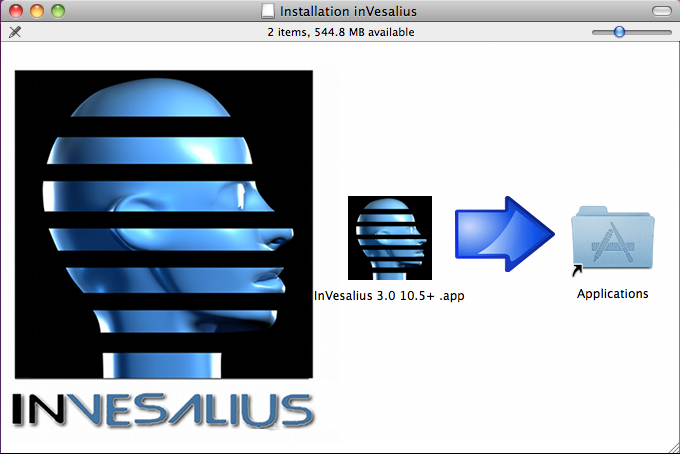
\includegraphics[scale=0.4]{mac2.png}
\end{figure}

Mantenha o botão esquerdo pressionado sobre o ícone do software InVesalius e arraste-o para o ícone \textit{Applications}
ambos contidos no instalador.

%\begin{figure}[!htb]
%\centering
%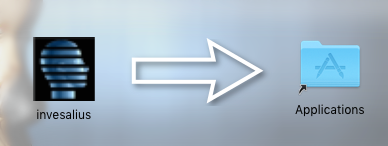
\includegraphics[scale=0.4]{mac4.png}
%\end{figure}

O software já encontra-se instalado, bastando acessar pelo menu

\chapter{Image import}

InVesalius imports files in DICOM format, including compressed files (lossless JPEG), Analyze (Mayo Clinic$^\copyright$), NIfTI, PAR/REC, BMP, TIFF, JPEG and PNG formats.

\section{DICOM}

Under the File menu, click on Import DICOM or use the shortcut Ctrl+I. Additionally, DICOM files can be imported by clicking on the icon shown in Figure~\ref{fig:import}.

\begin{figure}[!htb]
\centering

\includegraphics[scale=0.2]{../user_guide_figures/icons/file_import_original.png}
\caption{Shortcut to DICOM import}
\label{fig:import}
\end{figure}

\hspace{.2cm}

Select the directory containing the DICOM files, as in Figure~\ref{fig:win_folder}. InVesalius will search for files also in subdirectories of the chosen directory,
if they exist.

\newpage

Once the directory is selected, click \textbf{OK}.

\begin{figure}[!htb]
\centering
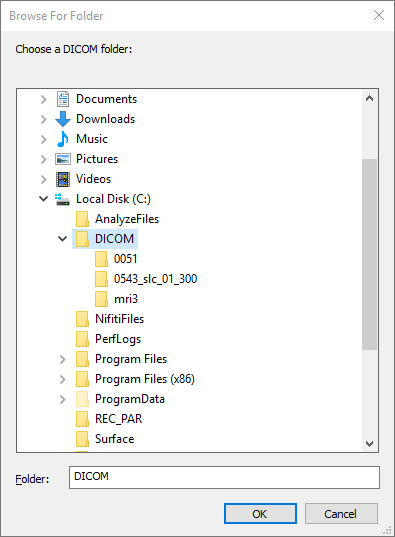
\includegraphics[scale=0.5]{../user_guide_figures/invesalius_screen/import_select_folder_en.png}
\caption{Folder Selection}
\label{fig:win_folder}
\end{figure}

\hspace{.2cm}

While InVesalius search for DICOM files in the directory, the loading progress of the scanned files is displayed, as shown in the Figure~\ref{fig:ver_file}.

\begin{figure}[!htb]
\centering
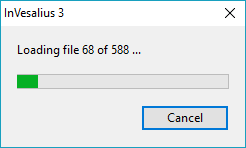
\includegraphics[scale=0.6]{../user_guide_figures/invesalius_screen/import_load_files_en.png}
\caption{Loading file status}
\label{fig:ver_file}
\end{figure}

\newpage

If DICOM files are found, a window open (shown Figure~\ref{fig:win_import}) will open to select the patient and respective series to be opened. It is also possible to skip images for reconstruction.

\begin{figure}[!htb]
\centering
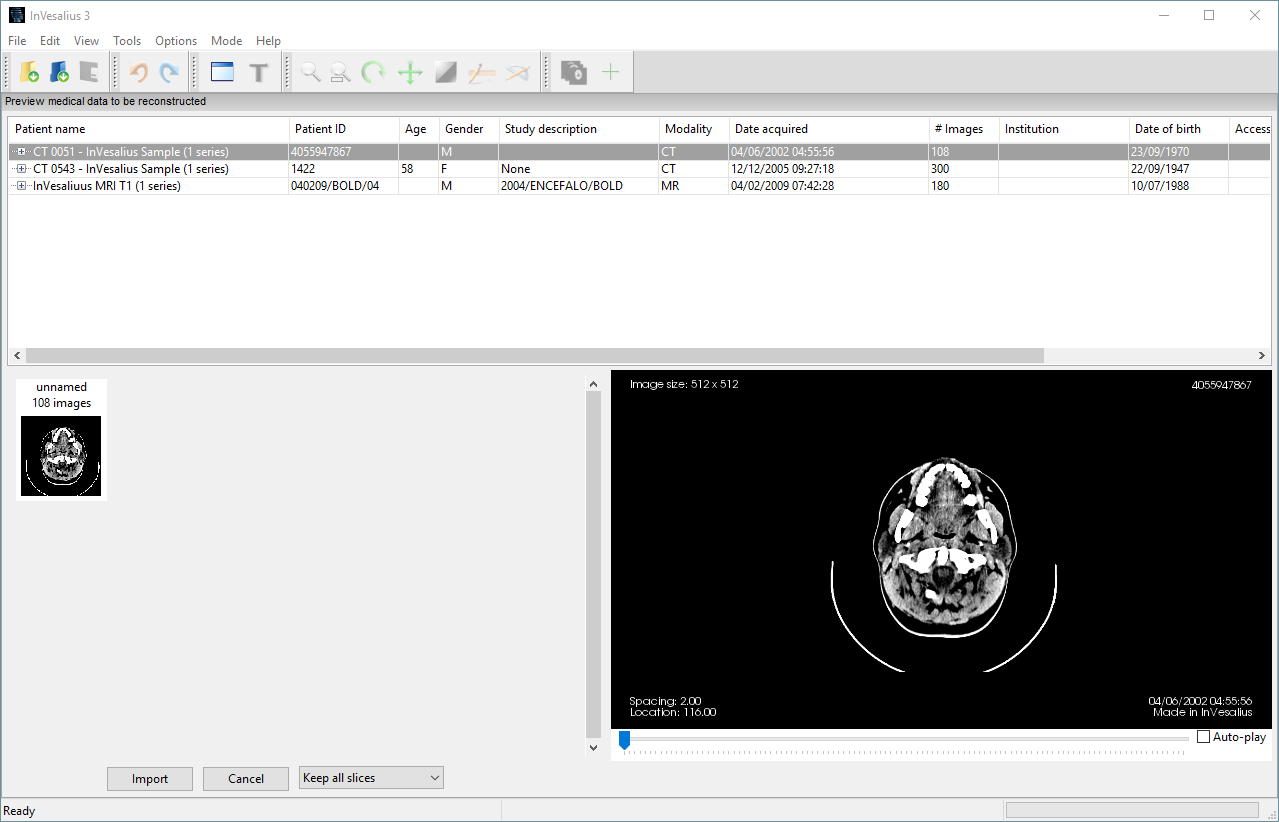
\includegraphics[scale=0.4]{../user_guide_figures/invesalius_screen/import_window_en.png}
\caption{Import window}
\label{fig:win_import}
\end{figure}

\newpage

To import a series with all images present, click "\textbf{$+$}" on the patient’s name to expand the corresponding series. Double-click on the description of the series. See Figure~\ref{fig:import_serie}.

\begin{figure}[!htb]
\centering
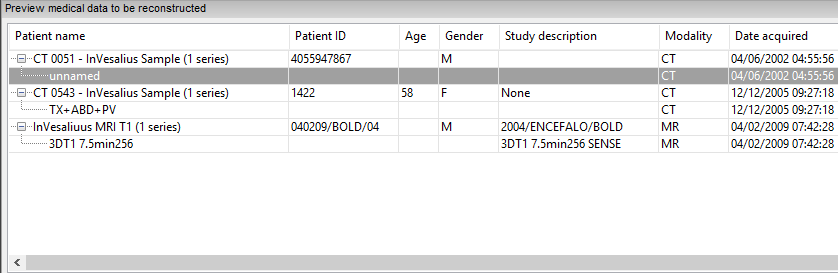
\includegraphics[scale=0.5]{../user_guide_figures/invesalius_screen/import_window_detail_en.png}
\caption{Series selection}
\label{fig:import_serie}
\end{figure}

In some cases, when there is no computer with memory and/or satisfactory processing to work with large numbers of images in a series, it is recommended to skip some of them. To do this, click \textbf{once} with the \textbf{left} mouse button over the description of the series (Figure~\ref{fig:import_serie}) and select how many images will be skipped (Figure~\ref{fig:skip_image}), then click \textbf{Import}.

\begin{figure}[!htb]
\centering
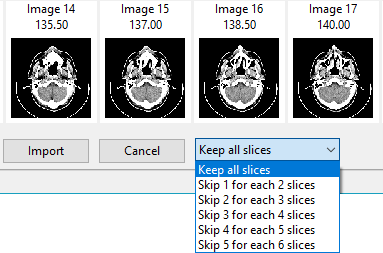
\includegraphics[scale=0.6]{../user_guide_figures/invesalius_screen/import_window_skip_slice_en.png}
\caption{Skip imagens option}
\label{fig:skip_image}
\end{figure}

If there is an insufficient amount of available memory at the time of loading the images it is recommended that the resolution of the slices be reduced to work with volumetric and surface visualization, as shown in Figure~\ref{fig:resize_image}.
The slices will be resized according to the percentage relative to the original resolution. For example, if each slice of the exam the dimension of 512 x 512 pixels and the "Percentage of original resolution" is suggested to be 60 \%, each resulting image will be 307 x 307 pixels. To open with the original pixel resolution, set the percentage to 100.

\begin{figure}[!htb]
\centering
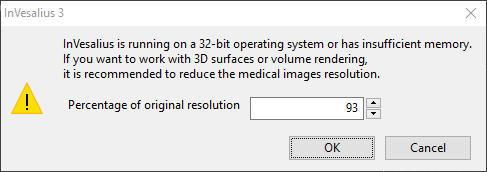
\includegraphics[scale=0.5]{../user_guide_figures/invesalius_screen/import_window_lower_memory_en.png}
\caption{Image size reduction}
\label{fig:resize_image}
\end{figure}

If the image was obtained with the gantry tilted it will be necessary to correct to avoid distortion of any reconstruction. InVesalius allows the user to do this easily. When importing an image with the gantry tilted a dialog will appear, showing the gantry tilt angle. (Figure~\ref{fig:gantry_tilt}). It is possible to change this value, but it is not recommended. Click on the \textbf{Ok} to do the correction. If you click on the \textbf{cancel} button the correction will not be done.

\begin{figure}[!htb]
\centering
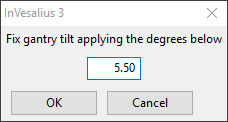
\includegraphics[scale=0.75]{../user_guide_figures/invesalius_screen/window_gantry_tilt_en.png}
\caption{Gantry tilt correction}
\label{fig:gantry_tilt}
\end{figure}

After the above procedure, a window will be displayed (Figure \ref{fig:prog_recons}) with reconstruction (when images are stacked and interpolated).

\begin{figure}[!htb]
\centering
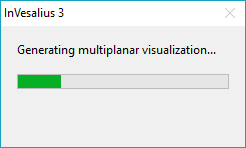
\includegraphics[scale=0.6]{../user_guide_figures/invesalius_screen/import_window_progress_en.png} 
\caption{Reconstruction progress}
\label{fig:prog_recons}
\end{figure}

\newpage

\section{Analyze}

To import Analyze files, under the \textbf{File} menu, click \textbf{Import other files}, then click in the \textbf{Analyze} option as show the Figure~\ref{fig:analyze_menu}.

\begin{figure}[!htb]
\centering
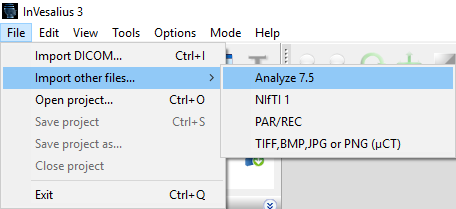
\includegraphics[scale=0.4]{../user_guide_figures/invesalius_screen/import_analyze_menu_en.png}
\caption{Menu for importing images in analyze format.}
\label{fig:analyze_menu}
\end{figure}

Select the Analyze file format (\textbf{.hdr}) and click on \textbf{Open} (Figure~\ref{fig:analyze_import}).
 
\begin{figure}[!htb]
\centering
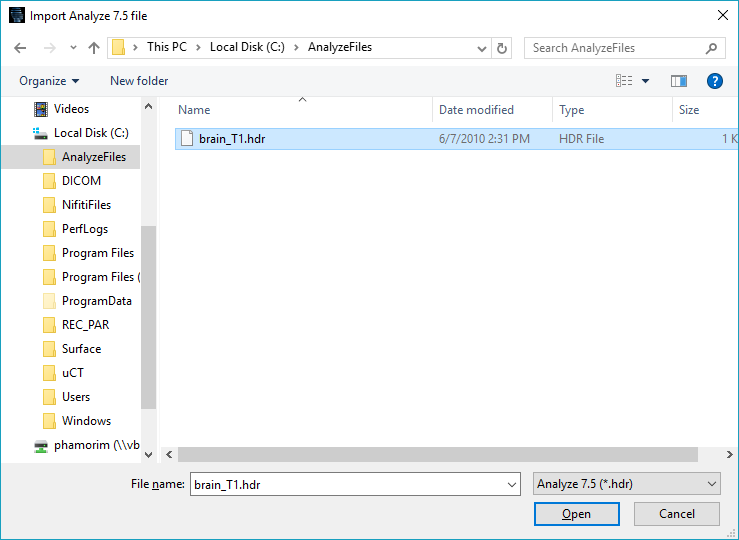
\includegraphics[scale=0.4]{../user_guide_figures/invesalius_screen/import_analyze_window_en.png}
\caption{Import analyze file format}
\label{fig:analyze_import}
\end{figure}

\section{NIfTI}

To import NIfTI files, under the \textbf{File}  menu, click \textbf{Import other files} and then click \textbf{NIfTI} as shown in Figure~\ref{fig:import_nifti_menu_pt}.


\begin{figure}[!htb]
\centering
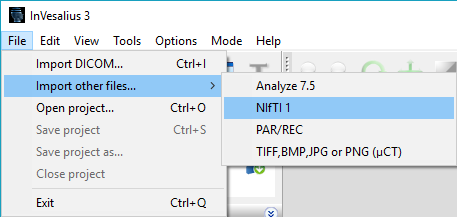
\includegraphics[scale=0.4]{../user_guide_figures/invesalius_screen/import_nifti_menu_en.png}
\caption{Menu to import images in NIfTI format}
\label{fig:import_nifti_menu_pt}
\end{figure}

Select the NIfTI file format, (either \textbf{nii.gz} or \textbf{.nii}) then click \textbf{Open} (Figure~\ref{fig:import_nifti_window_pt}). If the file is in another format as \textbf{.hdr}, select \textbf{all files(*.*)} option.

\begin{figure}[!htb]
\centering
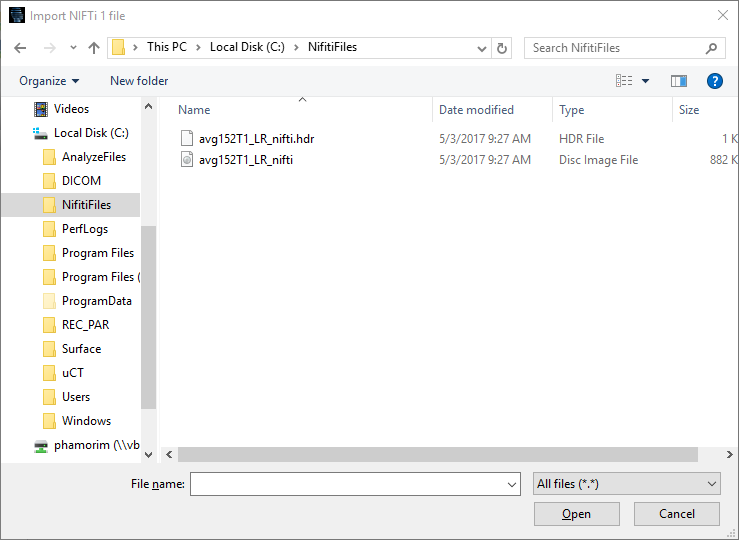
\includegraphics[scale=0.4]{../user_guide_figures/invesalius_screen/import_nifti_window_en.png}
\caption{Importing images in NIfTI format.}
\label{fig:import_nifti_window_pt}
\end{figure}

\section{PAR/REC}

To import PAR/REC file, under the \textbf{File} menu, click \textbf{Import other files}, and then click on \textbf{PAR/REC} as shown in Figure~\ref{fig:import_parrec_menu_pt}.

\begin{figure}[!htb]
\centering
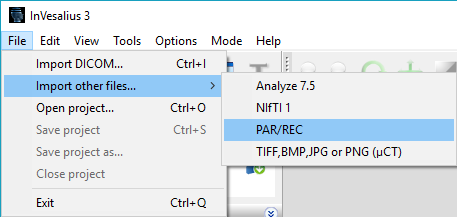
\includegraphics[scale=0.4]{../user_guide_figures/invesalius_screen/import_parrec_menu_en.png}
\caption{Menu for importing PAR/REC images}
\label{fig:import_parrec_menu_pt}
\end{figure}

Select PAR/REC file type, with the file extension \textbf{.par} and click \textbf{Open} (Figure~\ref{fig:import_parrec_window_pt}). If the file has no extension, select \textbf{all files(*.*)} option.

\begin{figure}[!htb]
\centering
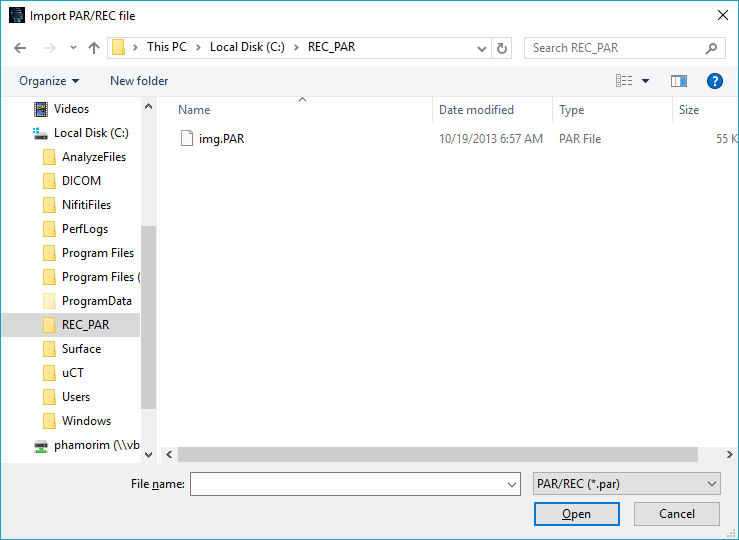
\includegraphics[scale=0.4]{../user_guide_figures/invesalius_screen/import_parrec_window_en.png}
\caption{PAR/REC import}
\label{fig:import_parrec_window_pt}
\end{figure}

\section{TIFF, JPG, BMP, JPEG or PNG (micro-CT)}

TIFF, JPG, BMP, JPEG or PNG file format for microtomography equipment (micro-CT or $\mu$CT) or others. InVesalius imports files in these formats if pixels present are represented in \textbf{grayscale}.

To import, click on menu \textbf{File}, \textbf{Import other files...} and then click on \textbf{TIFF, JPG, BMP, JPEG ou PNG ($\mu$CT)} option as shown the figure~\ref{fig:import_bmp_menu_pt}.

\begin{figure}[!htb]
\centering
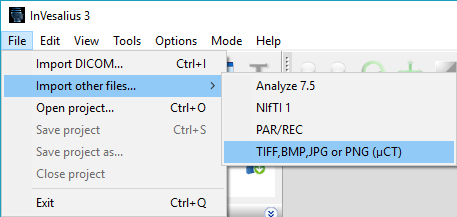
\includegraphics[scale=0.4]{../user_guide_figures/invesalius_screen/import_bmp_menu_en.png}
\caption{Import images in BMP and others formats}
\label{fig:import_bmp_menu_pt}
\end{figure}

Select the directory that contains the files, as shown the Figure~\ref{fig:import_bmp_select_folder}. InVesalius will search for files also in subdirectories of the chosen directory, if they exist. 

Click on \textbf{OK}.

\begin{figure}[!htb]
\centering
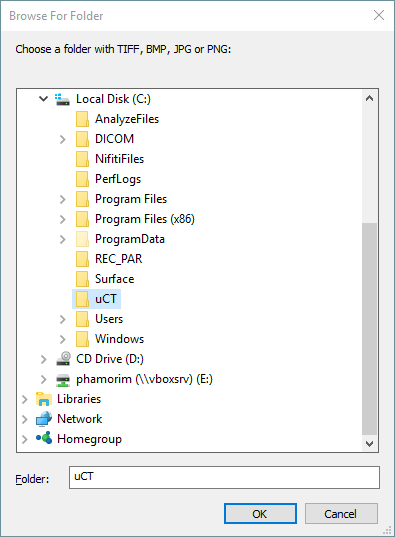
\includegraphics[scale=0.5]{../user_guide_figures/invesalius_screen/import_bmp_select_folder_en.png}
\caption{Folder selection}
\label{fig:import_bmp_select_folder}
\end{figure}

While InVesalius is looking for TIFF, JPG, BMP, JPEG, or PNG files in the directory, the upload progress of the scanned files is displayed, as illustrated in Figure~\ref{fig:import_bmp_load_pt}.

\begin{figure}[!htb]
\centering
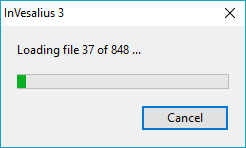
\includegraphics[scale=0.6]{../user_guide_figures/invesalius_screen/import_bmp_load_en.png}
\caption{Checking and loading files status.}
\label{fig:import_bmp_load_pt}
\end{figure}

If files in the desired formats are located, a window will open (shown in Figure~\ref{fig:import_bmp_window_pt}) to display the files eligible for reconstruction. Images can also be skipped to remove files from the rebuild list. The files are sorted according to file names. It is recommended that the files are numbered according to the desired rebuild order.

\begin{figure}[!htb]
\centering
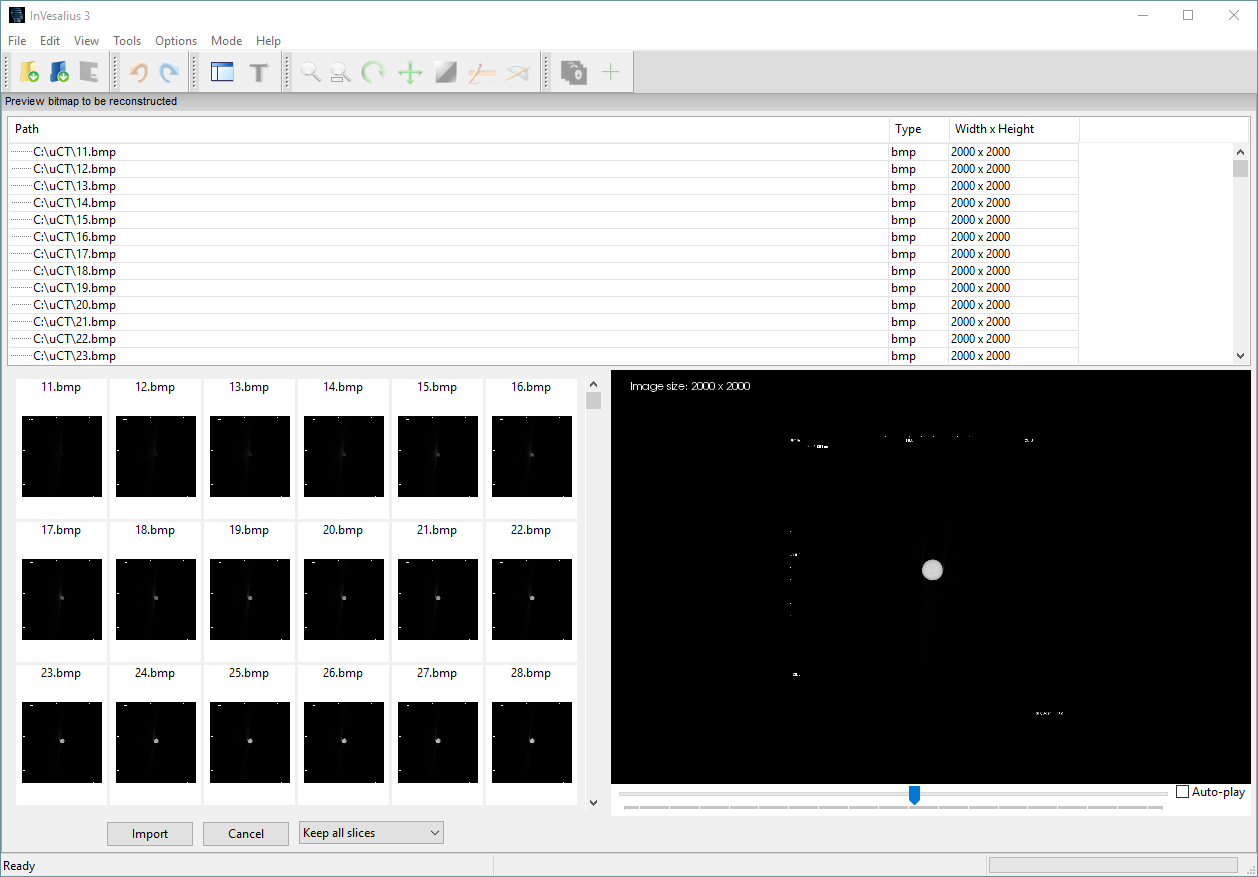
\includegraphics[scale=0.3]{../user_guide_figures/invesalius_screen/import_bmp_window_en.png}
\caption{Window to import BMP files.}
\label{fig:import_bmp_window_pt}
\end{figure}
 
To delete files that are not of interest, select a file by clicking the left mouse button and then pressing the delete key. You can also choose a
range of files to delete by clicking the \textbf{left mouse button} on a file, holding down the \textbf{shift} key, clicking again with the mouse button in the last file of the track and finally pressing the \textbf{delete} button.

Similar to when importing DICOM files, you can skip BMP images for re-building. In some cases, particularly where a computer with satisfactory memory and/or processing is unavailable, it may be advisable to skip some of them to retain adequate program functionality. To do this, select how many images to skip (Figure~\ref{fig:import_bmp_skip_pt}), then click \textbf{Import}.

\begin{figure}[!htb]
\centering
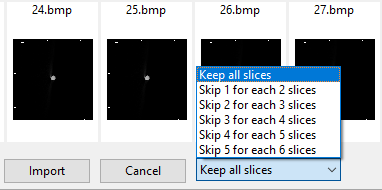
\includegraphics[scale=0.4]{../user_guide_figures/invesalius_screen/import_bmp_skip_en.png}
\caption{Importation window}
\label{fig:import_bmp_skip_pt}
\end{figure}

To reconstruct files of this type, a project name must be defined to indicate the orientation of the images (axial, coronal or sagittal), voxel spacing ($X$, $Y$ and $Z$) in \textbf{mm} as shown in the Figure~\ref{fig:import_bmp_spacing_pt}. The voxel spacing in $X$ is the pixel width of each image, $Y$ the pixel length, and $Z$ represents the distance of each slice (voxel height).

If the image set consists of microtomography images, more specifically GE and Brucker equipment, it is possible that InVesalius will read the text file with the acquisition parameters that normally stay in the same folder as the images and automatically insert the spacing. This verification can be done when the values of $X$, $Y$ and $Z$ are different from "1.00000000", otherwise it is necessary to enter the values of the respective spacing.

\textbf{Correct spacing is crucial for correctly importing objects in InVesalius. Incorrect spacing will provide incorrect measurements.}

Once all parameters have been input, click \textbf{OK}.

\begin{figure}[!htb]
\centering
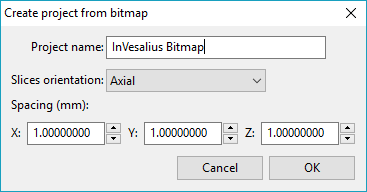
\includegraphics[scale=0.5]{../user_guide_figures/invesalius_screen/import_bmp_spacing_en.png}
\caption{Import Screen}
\label{fig:import_bmp_spacing_pt}
\end{figure}

If insufficient memory is available when loading images, it is recommended to reduce the resolution of the slices to work with volumetric and surface visualization, as shown in Figure~\ref{fig:import_bmp_resize_pt} window.The slices will be resized according to the percentage relative to the original resolution. For example, if each slice of the exam contains the dimension of $512 x 512$ pixels and the "Percentage of the original resolution" is suggested at 60, each resulting image will have $307 x 307$ pixels. If you want to open with the original resolution set the percentage to $100$.

\begin{figure}[!htb]
\centering
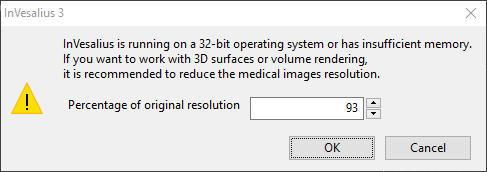
\includegraphics[scale=0.5]{../user_guide_figures/invesalius_screen/import_window_lower_memory_en.png}
\caption{Image resize}
\label{fig:import_bmp_resize_pt}
\end{figure}

After the previous steps, wait a moment for the program to complete the multiplanar reconstruction as shown in Figure~\ref{fig:import_bmp_mpr_pt.png}.

\begin{figure}[!htb]
\centering
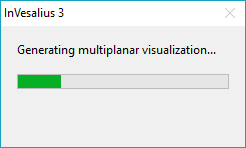
\includegraphics[scale=0.6]{../user_guide_figures/invesalius_screen/import_window_progress_en.png}
\caption{Multiplanar reconstruction in progress.}
\label{fig:import_bmp_mpr_pt.png}
\end{figure}

\chapter{Image adjustment}

InVesalius cannot guarantee the correct image order; images may contain incorrect information, or do not follow the DICOM standard. Therefore, it is recommended to check if a lesion or an anatomical mark is on the correct side. If not, it is possible to use the flip image or swap axes tools. For image alignment, the rotation image tool can be used.

It is possible to mirror the image. To do so, select the \textbf{Tools} menu, click \textbf{Image}, then \textbf{Flip} and click on one of the following options (Figure~\ref{fig:menu_img_mirroring_axis_pt}):

\begin{itemize}
	\item Right - Left
	\item Anterior - Posterior
	\item Top - Botton
\end{itemize}

\begin{figure}[!htb]
\centering
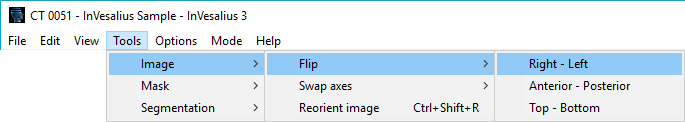
\includegraphics[scale=0.4]{menu_img_mirroring_axis_en.png}
\caption{Menu to activate flip image tool.}
\label{fig:menu_img_mirroring_axis_pt}
\end{figure}


Figure~\ref{fig:mirrored} shows a comparison between the input image and the flipped image. All other orientations are also modified when the image is flipped.

\begin{figure}[!htb]
  \centering
  \subfloat[Input image]{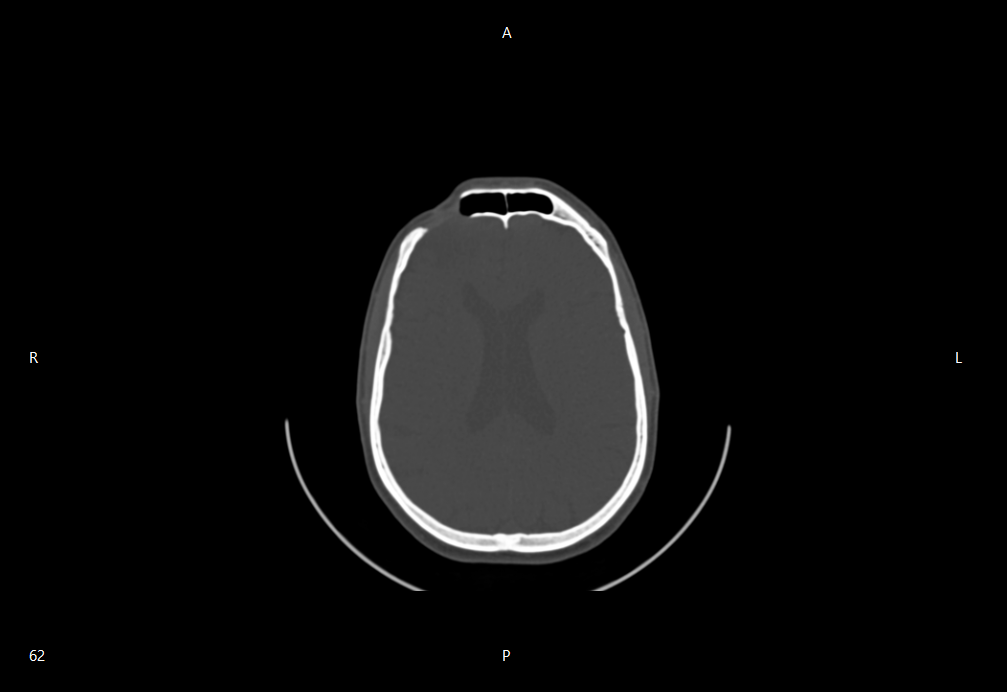
\includegraphics[width=0.45\textwidth]{mirror_axial_en.png}}  \qquad
  \subfloat[Flipped image]{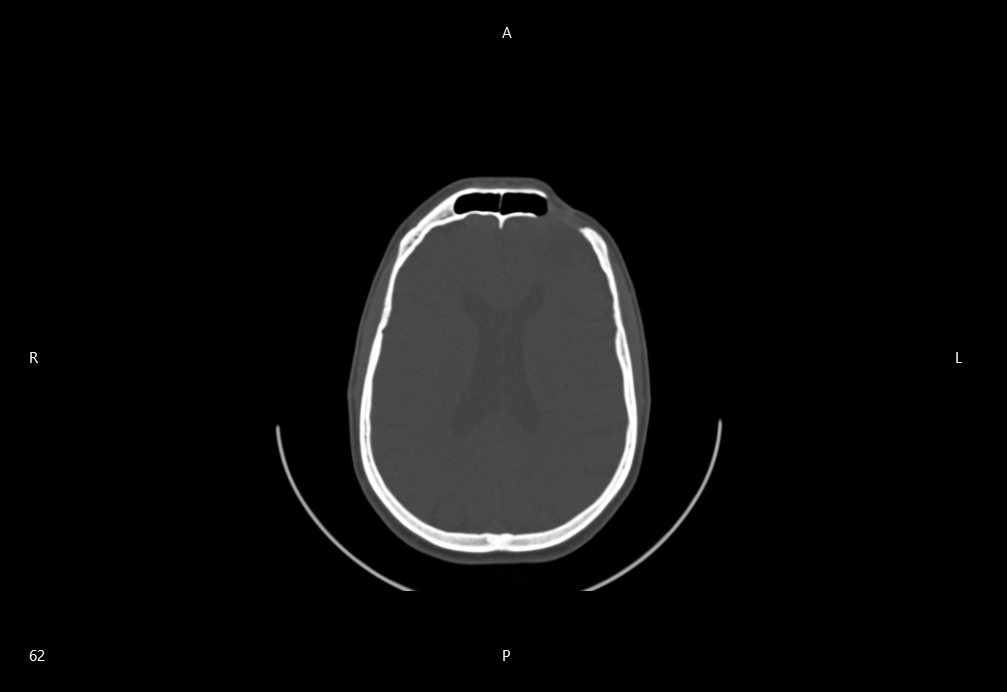
\includegraphics[width=0.45\textwidth]{mirror_axial_mirrored_en.png}}
  \hfill
  \caption{Example of a right-left flipped image.}
  \label{fig:mirrored}
\end{figure}

\section{Swap axes}

The swap axes tool changes the image orientation, in the case that the image has been wrongly imported. To perform this, select the \textbf{Tools} menu, click \textbf{Image}, then \textbf{Swap Axes} and click on one of the following options (Figure~\ref{fig:menu_invert_axis}):

\begin{itemize}
	\item From Right-Left to Anterior-Posterior
	\item From Right-Left to Top-Bottom
	\item From Anterior-Posterior to Top-Bottom
\end{itemize}


The Figures~\ref{fig:invert_axis_axial} and~\ref{fig:invert_axis_axial_inverted}, shows an example of an image with inverted axes.

\begin{figure}[!htb]
\centering
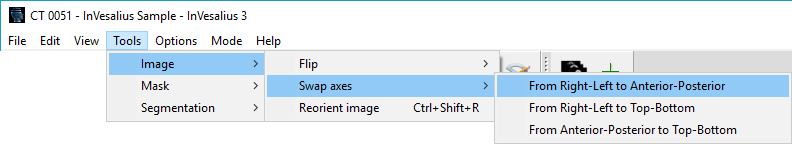
\includegraphics[scale=0.4]{menu_invert_axis_en.png}
\caption{Menu to activate swap image tool.}
\label{fig:menu_invert_axis}
\end{figure}

\begin{figure}[!htb]
\centering
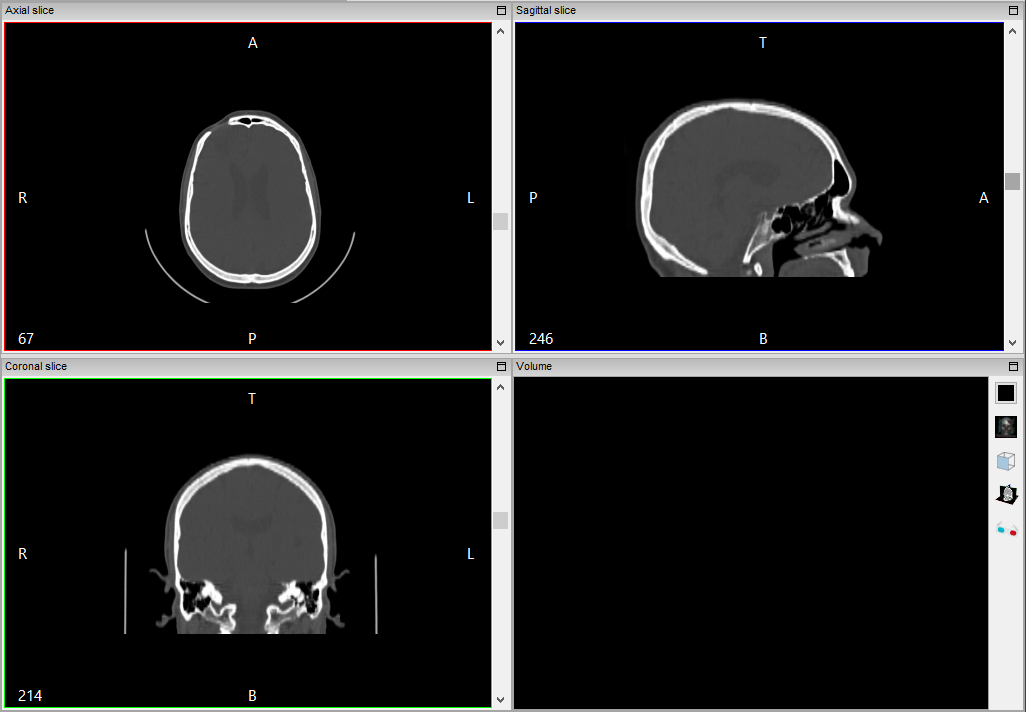
\includegraphics[scale=0.4]{invert_axis_axial_en.png}
\caption{Images before swap axes - from Anterior-Posterior to Top-Bottom.}
\label{fig:invert_axis_axial}
\end{figure}

\begin{figure}[!htb]
\centering
\includegraphics[scale=0.4]{invert_axis_axial_inverted_en.png}
\caption{Images after swap axes - from Anterior-Posterior to Top-Bottom.}
\label{fig:invert_axis_axial_inverted}
\end{figure}

\section{Reorient image (Rotate)}

If it is necessary to align the image with a certain point of reference, e.g. anatomical marker, use the reorient image tool. To open this tool select the \textbf{Tools} menu, click \textbf{Image}, then \textbf{Reorient Image} (Figure~\ref{fig:menu_img_reorient}).

\begin{figure}[!htb]
\centering
\includegraphics[scale=0.4]{menu_img_reorient_en.png}
\caption{Menu to activate reorient image tool.}
\label{fig:menu_img_reorient}
\end{figure}

When this tool is activated a window is opened (Figure~\ref{fig:image_reorient_window}) showing orientation and by how many degrees the image was rotated.

\begin{figure}[!htb]
\centering
\includegraphics[scale=0.7]{image_reorient_window_en.png}
\caption{Window that shows the reorientation image parameters.}
\label{fig:image_reorient_window}
\end{figure}

To start reorienting the image, define the interpolation method that will applied after rotation, by default is tricubic interpolation. The interpolation options are:

\begin{itemize}
	\item Nearest Neighbour
	\item Trilinear
	\item Tricubic
	\item Lanczos
\end{itemize}


Then, select the rotation point by keeping the \textbf{left} mouse button pressed between the two lines intersecting (Figure~\ref{fig:image_reorient_adjust_center}) at one orientation, e.g. axial, coronal or sagittal, and \textbf{drag} to the desired point.

\begin{figure}[!htb]
\centering
\includegraphics[scale=0.4]{image_reorient_adjust_center_en.png}
\caption{Defining the axis of rotation of the image.}
\label{fig:image_reorient_adjust_center}
\end{figure}

To rotate the image it is necessary to keep the \textbf{left} mouse button pressed and \textbf{drag} until the reference point or anatomical marker stays aligned with one of the lines (Figure~\ref{fig:image_reorient_rotated}). After the image is in the desired position, click \textbf{Apply} in the parameter window (Figure~\ref{fig:image_reorient_window}). This may take a few moments depending on the image size. Figure~\ref{fig:image_reorient_rotated_applied} shows an image successfully reoriented.

\begin{figure}[!htb]
\centering
\includegraphics[scale=0.4]{image_reorient_rotated_en.png}
\caption{Rotated image.}
\label{fig:image_reorient_rotated}
\end{figure}

\begin{figure}[!htb]
\centering
\includegraphics[scale=0.4]{image_reorient_rotated_applied_en.png}
\caption{Rotated image after reorientation is done.}
\label{fig:image_reorient_rotated_applied}
\end{figure}

\chapter{Manipulação de Imagens (2D)}

\section{Reconstrução Multiplanar}

Ao importar as imagens, o InVesalius mostra, automaticamente, a sua reconstrução
multiplanar nas orientações Axial, Sagital e Coronal, bem como uma janela para manipulação 3D.
Veja a figura \ref{fig:mpr}.

\begin{figure}[!htb]
\centering
\includegraphics[scale=0.30]{multiplanar_mask_window_pt.png}
\caption{Reconstrução multiplanar}
\label{fig:mpr}
\end{figure}

\newpage

Além de criar a reconstrução multiplanar, o InVesalius segmenta a imagem, destacando, por exemplo, os
ossos dos tecidos moles. O destaque é representado por meio da aplicação de cores sobre a estrutura
segmentada, isto é, as cores formam uma máscara sobre a imagem destacando a estrutura (figura
\ref{fig:mpr}). Isso será discutido em mais detalhes nos próximos capítulos.

Para esconder a máscara, usa-se o gerenciador de dados, localizado no canto inferior esquerdo
da tela. Basta escolher a aba \textbf{Máscaras} e clicar \textbf{uma} vez com o botão
\textbf{esquerdo} do mouse sobre o ícone do olho ao lado de \textbf{"Máscara 1"}. Veja a figura
\ref{fig:ger_masc}.

\begin{figure}[!htb]
\centering
\includegraphics[scale=0.8]{data_mask_pt.png}
\caption{Gerenciador de máscaras}
\label{fig:ger_masc}
\end{figure}

O ícone do olho desaparece, e as cores da máscara de segmentação são escondidas (figura
\ref{fig:mpr_sem_mask}).

\begin{figure}[!htb]
\centering
\includegraphics[scale=0.30]{multiplanar_window_pt.png}
\caption{Reconstrução multiplanar sem máscara de segmentação}
\label{fig:mpr_sem_mask}
\end{figure}

\subsection{Orientação axial}

A orientação axial é composta de cortes transversais da região
de interesse, ou seja, cortes paralelos ao plano axial do corpo humano.
Na figura \ref{fig:axial_corte}, é exibida uma imagem em orientação axial da
região do crânio.

\begin{figure}[!htb]
\centering
\includegraphics[scale=0.15]{axial.jpg}
\caption{Corte axial}
\label{fig:axial_corte}
\end{figure}

\subsection{Orientação sagital}

A orientação sagital é composta de cortes realizados lateralmente
em relação à região de interesse, ou seja, cortes paralelos ao plano sagital do corpo humano,
que o divide nas porções esquerda e direita.
A figura \ref{fig:sagital_slice} mostra uma imagem do crânio em orientação sagital.

\begin{figure}[!htb]
\centering
\includegraphics[scale=0.15]{sagital.jpg}
\caption{Corte sagital}
\label{fig:sagital_slice}
\end{figure}

\newpage

\subsection{Orientação coronal}

A orientação coronal é composta de cortes paralelos ao plano coronal,
que divide o corpo humano em metades ventral e dorsal.
A figura \ref{fig:coronal_slice} mostra uma imagem do crânio em orientação
coronal.

\begin{figure}[!htb]
\centering
\includegraphics[scale=0.15]{coronal.jpg}
\caption{Corte coronal}
\label{fig:coronal_slice}
\end{figure}


\section{Correspondência entre as orientações axial, sagital e coronal}
\label{sec:corresp_all_orient}

Para saber qual o ponto comum das imagens nas diferentes orientações, basta acionar o
recurso "Cruz de interseção de fatias" pelo ícone de atalho localizado na barra de ferramentas.
Veja a figura \ref{fig:cross_icon}.

\begin{figure}[!htb]
\centering
\includegraphics[scale=1]{cross.png}
\caption{Atalho para mostrar ponto comum entre diferentes orientações}
\label{fig:cross_icon}
\end{figure}

Quando o recurso é acionado, dois segmentos de reta que se cruzam perpendicularmente são exibidos
sobre cada imagem (figura \ref{fig:cross_all}). O ponto de interseção de cada par de segmentos
representa o ponto comum  entre as diferentes orientações.

\newpage

Para modificar o ponto, mantenha \textbf{pressionado} o botão \textbf{esquerdo} do mouse e o
\textbf{arraste}. Automaticamente, os pontos correspondentes serão atualizados em cada imagem.

\begin{figure}[!htb]
\centering
\includegraphics[scale=0.4]{multiplanar_window_cross_pt.png}
\caption{Ponto comum entre orientações diferentes}
\label{fig:cross_all}
\end{figure}

Para desativar a funcionalidade, basta clicar novamente sobre o atalho (figura \ref{fig:cross_icon}).
Esse recurso pode ser utilizado em conjunto com o editor de fatias (que será comentado mais à frente).


\section{Interpolação}

Por padrão a visualização das imagens 2D são interpoladas (figura~\ref{fig:interp}).a, caso deseja desativar esse recurso, basta ir no menu \textbf{Visualizar}, \textbf{Fatias interpoladas} (figura~\ref{fig:menu_interpoleted_image_pt}). Dessa forma será possível visualizar cada pixel individualmente como mostra a figura~\ref{fig:interp}.b. 

\textbf{Observação: Essa interpolação é apenas para efeitos de visualização, não influenciando diretamente na segmentação ou na geração de superfície 3D.}

\begin{figure}[!htb]
\centering
\includegraphics[scale=0.6]{menu_interpoleted_image_pt.png}
\caption{Menu para desativar e ativar interpolação}
\label{fig:menu_interpoleted_image_pt}
\end{figure}


\begin{figure}[!htb]
  \centering
  \subfloat[Interpolada]{\includegraphics[width=0.4\textwidth]{axial_interpoleted.png}}  \qquad
  \subfloat[Não interpolada]{\includegraphics[width=0.4\textwidth]{axial_not_interpoleted.png}}
  \hfill
  \caption{Visualização de imagem interpolada e não interpolada.}
  \label{fig:interp}
\end{figure}

\section{Mover}

Para mover uma imagem na tela, pode-se utilizar o ícone do atalho "Mover" da barra de ferramentas (figura
\ref{fig:move_icon}). Clique sobre o ícone para ativar o recurso e, em seguida, com o botão
\textbf{esquerdo} do mouse pressionado sobre a imagem, \textbf{arraste-a} para a direção desejada.
A figura \ref{fig:move_img} mostra uma imagem deslocada (movida).

\begin{figure}[!h]
\centering
\includegraphics[scale=0.25]{tool_translate_original.png}
\caption{Atalho para mover imagens}
\label{fig:move_icon}
\end{figure}

\begin{figure}[!h]
\centering
\includegraphics[scale=0.15]{axial_pan.jpg}
\caption{Imagem deslocada}
\label{fig:move_img}
\end{figure}

\section{Rotacionar}

A rotação de imagens pode ser ativada pelo ícone do atalho "Rotacionar" da barra de ferramentas (figura
\ref{fig:rot_icon}). Para rotacionar uma imagem, clique sobre o ícone e, em seguida, com o botão
\textbf{esquerdo} do mouse pressionado sobre a imagem, \textbf{arraste-a} no sentido horário ou
anti-horário, dependendo do sentido de rotação desejado.

\begin{figure}[!h]
\centering
\includegraphics[scale=0.25]{tool_rotate_original.png}
\caption{Atalho para rotacionar imagens}
\label{fig:rot_icon}
\end{figure}

\begin{figure}[!h]
\centering
\includegraphics[scale=0.15]{axial_rotate.jpg}
\caption{Imagem rotacionada}
\label{fig:rotate_all}
\end{figure}

\section{Ampliar (\textit{Zoom})}

No InVesalius, existem diferentes formas de ampliar uma imagem. Pode-se maximizar a janela da
orientação desejada, aplicar o \textit{zoom} diretamente na imagem, ou selecionar a região da imagem
que será ampliada.


\subsection{Maximizando as janelas de orientação}

Como já sabemos, a janela principal do InVesalius é dividida em 4 subjanelas: axial, sagital, coronal
e 3D. Cada uma delas pode ser maximizada de modo a ocupar toda a área da janela principal. Para isso,
basta clicar com o botão \textbf{esquerdo} do mouse no ícone existente no \textbf{canto superior direito}
da subjanela (figura \ref{fig:maximize_window}). Para restaurar uma janela maximizada a seu tamanho
anterior, basta clicar novamente no ícone.

\begin{figure}[!htb]
\centering
\includegraphics[scale=0.6]{maximize_sagital_mpr.png}
\caption{Detalhe de uma subjanela (Observe o ícone de maximizar no canto superior direito)}
\label{fig:maximize_window}
\end{figure}

\subsection{Ampliando ou reduzindo uma imagem}

Para ampliar ou reduzir uma imagem, clique sobre o ícone do atalho "\textit{Zoom}" na barra de
ferramentas (figura \ref{fig:zoom_icon}). Mantenha o botão \textbf{esquerdo} pressionado sobre
a imagem e \textbf{arraste} o mouse para \textbf{cima}, caso deseje ampliá-la, ou para \textbf{baixo},
caso deseje reduzi-la.

\begin{figure}[!htb]
\centering
\includegraphics[scale=0.25]{tool_zoom_original.png}
\caption{Atalho de \textit{Zoom}}
\label{fig:zoom_icon}
\end{figure}

\subsection{Ampliando uma área da imagem}

Para ampliar uma área determinada da imagem, clique sobre o ícone do atalho "Zoom baseado na seleção" 
na barra de ferramentas (figura \ref{fig:zoom_icon_loc}). Posicione o ponteiro do mouse na posição
inicial da seleção, clique e mantenha o botão \textbf{esquerdo} do mouse pressionado e \textbf{arraste-o}
até a posição final da seleção, formando um retângulo (figura \ref{fig:zoom_select}). Assim que o
botão esquerdo do mouse for liberado, a operação de \textit{zoom} será aplicada à região selecionada
(figura \ref{fig:zoom_applied}).

\begin{figure}[!htb]
\centering
\includegraphics[scale=0.25]{tool_zoom_select_original.png}
\caption{Atalho de \textit{Zoom} baseado na seleção}
\label{fig:zoom_icon_loc}
\end{figure}

\begin{figure}[!htb]
\centering
\includegraphics[scale=0.15]{tool_zoom_select_image.jpg}
\caption{Área selecionada para \textit{zoom}}
\label{fig:zoom_select}
\end{figure}

\begin{figure}[!htb]
\centering
\includegraphics[scale=0.15]{tool_image_with_zoom.jpg}
\caption{Imagem ampliada}
\label{fig:zoom_applied}
\end{figure}


\section{Brilho e contraste (Janelas)}
\label{sec:ww_wl}

Para melhorar a visualização das imagens, podemos utilizar o recurso de \textit{window width} e
\textit{window level}, popularmente conhecido por "brilho e contraste" ou "janela" (para radiologistas). 
Com esse recurso, é possível definir a faixa da escala de cinza (\textit{window level}) e a
largura dessa faixa (\textit{window width}) que serão usadas para exibir as imagens.

O recurso pode ser acionado pelo ícone do atalho "Contraste" na barra de ferramentas. Veja a figura \ref{fig:window_level_shortcut}.

\begin{figure}[!htb]
\centering
\includegraphics[scale=0.70]{tool_contrast_original.png}
\caption{Atalho de brilho e contraste}
\label{fig:window_level_shortcut}
\end{figure}

Para aumentar o brilho, mantenha o botão \textbf{esquerdo} do mouse pressionado e o \textbf{arraste} na 
horizontal para a direita. Para diminuir o brilho, basta arrastar o mouse para a esquerda. O contraste
pode ser alterado arrastando o mouse (com o botão \textbf{esquerdo} pressionado) na vertical: para cima
para aumentar, ou para baixo para diminuir o contraste.

Para desabilitar o recurso, clique novamente sobre o ícone do atalho (figura \ref{fig:window_level_shortcut}).

É possível utilizar padrões pré-definidos de brilho e contraste. A tabela \ref{tab:window_level} relaciona
alguns tipos de tecido com os respectivos valores de brilho e contraste da imagem. Para usar um padrão
pré-definido, posicione o cursor do mouse sobre a imagem e clique com o botão \textbf{direito} para abrir um
menu de contexto sobre ela. Quando o menu se abrir, selecione a entrada \textbf{Brilho e Contraste} e, em
seguida, clique sobre a opção pré-definida, de acordo com o tipo de tecido, como mostra a figura
\ref{fig:window_level}.


\begin{figure}[!htb]
\centering
\includegraphics[scale=0.40]{menu_window_and_level_pt.png}
\caption{Menu de contexto para seleção de brilho e contraste}
\label{fig:window_level}
\end{figure}

\begin{table}[h]
\centering
\caption{Valores de brilho e contraste para alguns tecidos}
\begin{tabular}{lcc}\\
\hline % este comando coloca uma linha na tabela
Tecido & Brilho & Contraste\\
\hline
\hline
Padrão & Exame & Exame\\
Manual & Alterado & Alterado\\
Abdômen & 350 & 50 \\
Cérebro & 80 & 40\\
Enfisema & 500 & -850\\
Fossa Posterior Nasal & 120 & 40\\
Fígado & 2000 & -500\\
Isquemia - Contraste Tecidos Duros & 15 & 32\\
Isquemia - Contraste Tecidos Moles & 80 & 20\\
Laringe & 180 & 80\\
Mediastino & 350 & 25\\
Osso & 2000 & 300\\
Pélvis & 450 & 50\\
Pulmão Duro & 1000 & -600\\
Pulmão Mole & 1600 & -600\\
Seio & 4000 & 400\\
Vascular - Duro & 240 & 80\\
Vascular - Mole & 680 & 160\\
\hline
\end{tabular}
\label{tab:window_level}
\end{table} 

\begin{figure}
  \centering
  \subfloat[Osso]{\label{fig:contrast_bone}\includegraphics[width=0.4\textwidth]{contraste_osso}} \qquad          
  \subfloat[Pulmão]{\label{fig:contrast_isq}\includegraphics[width=0.4\textwidth]{contraste_pulmao}}
  \caption{Diferentes tipos de brilho e constraste}
  \label{fig:two_window_level}
\end{figure}


\section{Pseudocor}

Outro recurso para melhorar a visualização das imagens são as pseudocores. Elas substituem os níveis
de cinza por cores, ou pelos níveis de cinza invertidos. Nesse último caso, regiões da imagem que
antes eram mais claras se tornam mais escuras e vice-versa.

Para alterar a visualização usando uma pseudocor, posicione o cursor do mouse sobre a imagem e clique
com o botão \textbf{direito} para abrir um menu de contexto sobre ela. Quando o menu se abrir,
selecione a entrada \textbf{Pseudocor} e, em seguida, clique sobre a opção de pseudocor desejada, como
mostra a figura \ref{fig:pseudo_color}.

\begin{figure}[H]
\centering
\includegraphics[scale=0.40]{pseudo_menu_pt.png}
\caption{Pseudo Cor}
\label{fig:pseudo_color}
\end{figure}

As figuras de \ref{fig:image_default} a \ref{fig:image_saturation} exemplificam as diversas opções de
pseudocor disponíveis.

\begin{figure}[h]
  \centering
  \subfloat[Default]{\label{fig:image_default}\includegraphics[width=0.25\textwidth]{pseudo_default.jpg}} \qquad
  \subfloat[Inverted Gray Image]{\label{fig:image_inverted}\includegraphics[width=0.25\textwidth]{pseudo_inverse.jpg}} \qquad
  \subfloat[Rainbow]{\label{fig:image_arc}\includegraphics[width=0.25\textwidth]{pseudo_rainbow.jpg}} \\
  \subfloat[Desert]{\label{fig:image_desert}\includegraphics[width=0.25\textwidth]{pseudo_desert.jpg}} \qquad
  \subfloat[Hue]{\label{fig:image_matiz}\includegraphics[width=0.25\textwidth]{pseudo_hue.jpg}} \qquad
  \subfloat[Ocean]{\label{fig:image_ocean}\includegraphics[width=0.25\textwidth]{pseudo_ocean.jpg}}\\
\subfloat[Saturation]{\label{fig:image_saturation}\includegraphics[width=0.25\textwidth]{pseudo_saturation.jpg}}  
  \caption{Alguns tipos diferentes de pseudo-cor}
  \label{fig:pseudo_color_types}
\end{figure}

\newpage

\section{Tipo de projeção}

É possível alterar o tipo de projeção das imagens 2D a serem visualizadas, além do modo normal, o InVesalius dispõe de seis tipos de projeções que podem serem acessadas da seguinte forma: Possicione o cursor do mouse sobre a imagem e clique com o botão \textbf{direito} para abrir um menu de contexto sobre ela. Quando o menu se abrir, selecione a entrada tipo de projeção e, em seguida, clique sobre a opção de pseudocor desejada, como mostra a figura~\ref{fig:menu_proj}.

\begin{figure}[H]
\centering
\includegraphics[scale=0.60]{menu_projection_pt.png}
\caption{Menu de Tipo de projeção}
\label{fig:menu_proj}
\end{figure}

\subsection{Normal}

O modo normal é a visualização padrão, ou seja, sem nenhum tipo de projeção, da maneira em que a imagem foi adquirida ou customizada previamente seja com brilho e contraste ou pseudocor. Exemplificamos na figura~\ref{fig:proj_normal}.

\begin{figure}[H]
\centering
\includegraphics[scale=0.40]{multiplanar_window_pt.png}
\caption{Projeção normal}
\label{fig:proj_normal}
\end{figure}

\subsection{MaxIP}
\label{sec:max_ip}
MaxIP também é conhecido como MIP (\textit{Maximum Intensity Projection}), o método seleciona somente os voxels que possuem intensidade máxima entre os visitados como mostra a figura~\ref{fig:proj_maxip}. De acordo com a quantidade ou "profundidade" do MaxIP cada voxel é visitado em ordem de sobreposição, por exemplo, para selecionar MaxIP do pixel $(0,0)$ composto por 3 fatias é necessário visitar o pixel $(0,0)$ das fatias $(1,2,3)$ e selecionar o maior valor.

\begin{figure}[H]
\centering
\includegraphics[scale=0.40]{multiplanar_window_maxip_pt.png}
\caption{Projeção MaxIP ou MIP}
\label{fig:proj_maxip}
\end{figure}

Como mostra a figura~\ref{fig:proj_maxip_qtd}, a quantidade de imagens que irá compor o MaxIP é setada no inferior da imagem de cada orientação.

\begin{figure}[H]
\centering
\includegraphics[scale=0.80]{multiplanar_window_maxip_number_pt.png}
\caption{Seleção da quantidade de imagens que compõe o MaxIP ou MIP}
\label{fig:proj_maxip_qtd}
\end{figure}

\subsection{MinIP}

Ao contrário do MaxIP, o MinIP (\textit{Minimum Intensity Projection}) seleciona somente os voxels que possuem internsidade minima entre os visitados, apresentamos na figura~\ref{fig:proj_minIP} um exemplo. A seleção da quantidade de imagens que irá compor a projeção é feita no inferior da imagem de cada orientação como mostra a figura~\ref{fig:proj_maxip_qtd}.

\begin{figure}[H]
\centering
\includegraphics[scale=0.40]{multiplanar_window_minip_pt.png}
\caption{Projeção MinIP}
\label{fig:proj_minIP}
\end{figure}

\subsection{MeanIP}
A técnica MeanIP (\textit{Mean Intensity Projection}) que é mostrada na figura~\ref{fig:proj_meanIP} compõe a projeção realizando a média dos voxels visitados. Os voxels são visitados da mesma forma dos métodos MaxIP e MinIP. Também é possível definir quantas imagens irão compor a projeção no inferior da imagem de cada orientação como é mostrada na figura~\ref{fig:proj_maxip_qtd}.

\begin{figure}[H]
\centering
\includegraphics[scale=0.40]{multiplanar_window_mean_pt.png}
\caption{Projeção MeanIP}
\label{fig:proj_meanIP}
\end{figure}

\subsection{MIDA}
\label{sub:mida}
A técnica MIDA (\textit{Maximum Intensity Difference Accumulation}) projeta uma imagem levando em consideração somente os voxels que possuem valores máximos locais. A partir de cada pixel da tela é simulado um raio em direção ao volume, cada voxel é interceptado por cada um destes raios chegando até o final do volume, cada um desses voxels visitados tem o seu valor acumulado, mas são levados em consideração somente se o valor for maior que os valores já visitados anteriormente. A exemplo do MaxIP, é possível selecionar quantas imagens serão utilizadas para acumular os valores. Apresentamos na figura~\ref{fig:proj_MIDA} um exemplo de projeção MIDA.  

\begin{figure}[H]
\centering
\includegraphics[scale=0.40]{multiplanar_window_mida_pt.png}
\caption{Projeção MIDA}
\label{fig:proj_MIDA}
\end{figure}

Como mostra a figura~\ref{fig:proj_MIDA_inv}, é possível inverter a ordem que os voxels são visitados, bastando selecionar a opção \textbf{Ordem invertida} no canto inferior da tela.

\begin{figure}[H]
\centering
\includegraphics[scale=0.40]{multiplanar_window_mida_inverted_pt}
\caption{Projeção MIDA em ordem invertida}
\label{fig:proj_MIDA_inv}
\end{figure}

\subsection{Contorno MaxIP}

Compõe a projeção 2D do conjunto de imagens que contém o volume usando a técnica \textit{Contour MaxIP}. A técnica consiste em visualizar contornos presentes na projeção gerada com a técnica MaxIP(\ref{sec:max_ip}). Um exemplo é apresentado na figura~\ref{fig:proj_contorno_maxip}.

\begin{figure}[H]
\centering
\includegraphics[scale=0.40]{multiplanar_window_contour_maxip_pt.png}
\caption{Projeção de Contorno MaxIP}
\label{fig:proj_contorno_maxip}
\end{figure}

\subsection{Contorno MIDA}

Compõe a projeção 2D do conjunto de imagens que contém o volume usando a técnica \textit{Contour MIDA}. A técnica consiste em visualizar contornos presentes na projeção gerada com a técnica MIDA(\ref{sub:mida}). A exemplo do MIDA é possível inverter a ordem que o volume é visitado. Exemplificamos na figura~\ref{fig:proj_contorno_mida}.

\begin{figure}[H]
\centering
\includegraphics[scale=0.40]{multiplanar_window_contour_mida_pt.png}
\caption{Projeção de Contorno MIDA}
\label{fig:proj_contorno_mida}
\end{figure}

\chapter{Segmentation}

To select a certain type of tissue from an image it's used the segmentation feature at InVesalius.

\section{Threshold}

Limiar é uma técnica de segmentação de imagens que permite selecionar da imagem somente os \textit{pixels} cuja intensidade está dentro de um limiar definido pelo usuário.  O limiar é definido por dois números, limiares inicial e final, também conhecidos como \textit{thresholds} mínimo e máximo. Como referência para a definição, é utilizada a escala de Hounsfield (tabela \ref{tab:escala_hounsfield}).

In thresholding segmentation technique only the \textit{pixels} whose intensity is inside threshold range defined by the user. Threshold is defined by two number, the initial and final threshold, also known as minimum and maximum threshold. ...

Thresholding segmentation is located at the InVesalius left-panel, item \textbf{2. Select region of interest} (figure~\ref{fig:region_selection}).

\begin{figure}[!htb]
\centering
\includegraphics[scale=0.7]{segmentation_threshold_window_left_en.png}
\caption{Select region of interest - Threshold}
\label{fig:region_selection}
\end{figure}

Before starting segment it's necessary to configure a mask. A mask is a image overlayed to exam image where the selected regions are colored. See figure~\ref{fig:region_selection_masc}

\begin{figure}[!htb]
\centering
\includegraphics[scale=0.4]{segmentation_threshold_axial_en.png}
\caption{Mask - selected region in yellow.}
\label{fig:region_selection_masc}
\end{figure}

To change the threshold you may use the control that represents the image grayscale (figure~\ref{fig:region_selection_bar}). Move the \textit{left} sliding control to change the initial threshold. Move the \textit{right} sliding control to change the final threshold. It's also possible to to digit the desired threshold values in the text boxes in the left and right side of the thresholding control. Changing the thresholding values, automatically the mask will be updated, showing with a color the \textit{pixel} that are inside the thresholding range.


\begin{figure}[!htb]
\centering
\includegraphics[scale=0.75]{segmentation_threshold_bar.png}
\caption{Selecting the \textit{pixels} with intensity between $226$ and $3021$ (Bone)}
\label{fig:region_selection_bar}
\end{figure}

It's also possible to select some predefined thresholding values based on some type of tissues, like displayed in the figure~\ref{fig:limiar_presets}. Just select the desired tissue and the mask automatically updated.

\begin{figure}[!htb]
\centering
\includegraphics[scale=0.65]{segmentation_threshold_presets_en.png}
\caption{Selection list with some predefined thresholding values.}
\label{fig:limiar_presets}
\end{figure}

The table~\ref{tab:limiar} show thresholding values according to some tissues or materials.

\begin{table}[h]
\centering
\caption{Predefined thresholding values to some materials}
\begin{tabular}{lcc}\\
\hline % este comando coloca uma linha na tabela
Material & Initial threshold & Final Threshold\\
\hline
\hline
Bone & 226 & 3021\\
Compact Bone (Adult) & 662 & 1988\\
Compact Bone (Child) & 586 & 2198\\
Custom & User Def. & User Def.\\
Enamel (Adult) & 1553 & 2850\\
Enamel (Child) & 2042 & 3021\\
Fat Tissue (Adult) & -205 & -51\\
Fat Tissue (Child) & -212 & -72\\
Muscle Tissue (Adult) & -5 & 135\\
Muscle Tissue (Child) & -25 & 139\\
Skin Tissue (Adult) & -718 & -177\\
Skin Tissue (Child) & -766 & -202\\
Soft Tissue & -700 & 225\\
Spongial Bone (Adult) & 148 & 661\\
Spongial Bone (Child) & 156 & 585\\
\hline
\end{tabular}
\label{tab:limiar}
\end{table}
\newpage

The table~\ref{tab:limiar} is indicated to images obtained from medical tomographs. The range of gray values from images obtained from odontological tomographs are greater and non-regular. Thus, it's necessary to use sliding control (figure~\ref{fig:region_selection_bar}) to adjust the thresholding values.

If you want to create a new mask click on the button \textbf{Create new mask} inside the item  \textbf{2. Select region of interest}. See the figure~\ref{fig:shortcut_new_mask}.

\begin{figure}[!htb]
\centering
\includegraphics[scale=0.2]{object_add_original}
\caption{Button to create a new mask.}
\label{fig:shortcut_new_mask}
\end{figure}

Clicando-se nesse atalho, uma nova janela será apresentada (figure \ref{fig:create_new_mask}).  Selecione a faixa de limiar desejada e clique em \textbf{OK}.

After clicking on this button a dialog will be shown (figure~\ref{fig:create_new_mask}). Select the desired threshold and click on \textbf{Ok}.

\begin{figure}[!htb]
\centering
\includegraphics[scale=0.55]{segmentation_threshold_window_dialog_en.png}
\caption{Creating a new mask.}
\label{fig:create_new_mask}
\end{figure}

\newpage

After the segmentation it's possible to generate a corresponding 3D surface. The surface is formed by triangles. The following chapter will give more details about surfaces.

Click on the \textbf{Create surface} button (figure~\ref{fig:generate_surface}) to create a new surface. If there is a surface created previously you may overwrite it with the new one. To do this select the option \textbf{Overwrite last surface} before creating the new surface.

\begin{figure}[!htb]
\centering
\includegraphics[scale=0.55]{segmentation_generate_surface_en.png}
\caption{Create surface button.}
\label{fig:generate_surface}
\end{figure}

After a few moments the surface will be displayed at the 3D visualization window of InVesalius (figure~\ref{fig:surface}).

\begin{figure}[!htb]
\centering
\includegraphics[scale=0.5]{surface_from_threshold.png}
\caption{3D surface.}
\label{fig:surface}
\end{figure}



\section{Manual segmentation (Image edition)}

Thresholding segmentation may not be efficient in some case since it's applied to the whole image. Manual segmentation may be used o segment only an isolated image region. Manual segmentation turns possible to add or remove some image regions to the segmentation. Manual segmentation requires more knowledge of  human anatomy. To use it click on \textbf{Manual edition} (figure~\ref{fig:advanced_edition}) to open the manual segmentation panel.

\begin{figure}[!htb]
\centering
\includegraphics[scale=0.75]{segmentation_manual_label_en.png}
\caption{Icon to open the Manual segmentation panel.}
\label{fig:advanced_edition}
\end{figure}

Figure~\ref{fig:edition_slices_ref} show the Manual segmentation panel.

\begin{figure}[!htb]
\centering
\includegraphics[scale=0.6]{segmentation_manual_window_en.png}
\caption{Manual segmentation panel.}
\label{fig:edition_slices_ref}
\end{figure}

There are two brushes used to segmentation: a circle and a square. Click on triangle icon (see figure~\ref{fig:brush_type}) to and click on the desired brush.

\begin{figure}[!htb]
\centering
\includegraphics[scale=0.9]{segmentation_manual_pencil_type.png}
\caption{Brush types.}
\label{fig:brush_type}
\end{figure}

\newpage

It's also possible to adjust the brush size, like shown in the figure~\ref{fig:select_diameter}.

\begin{figure}[!htb]
\centering
\includegraphics[scale=0.8]{segmentation_manual_diameter.png}
\caption{Adjusting the brush size.}
\label{fig:select_diameter}
\end{figure}

It's needed to select the operation to be performed by the brush. These are the options:

\textbf{Draw}: to add a non-selected region to the segmentation;

\textbf{Erase}: to remove a selected region from the segmentation;

\textbf{Threshold}: applies the thresholding locally, adding or removing a
region if in inside or outside of the threshold range.

Figure~\ref{fig:select_brush_operations} shows the operations.

\begin{figure}[!htb]
\centering
\includegraphics[scale=0.7]{segmentation_manual_pencil_type_operation_type_en.png}
\caption{Brush operations}
\label{fig:select_brush_operations}
\end{figure}

Figure~\ref{fig:noise_amalgaman} shows a image with noises caused by the presence of dental prosthesis. See the rays emerging from the dental arch. The thresholding segments the noise since its intensity is inside of the threshold of bone.

\begin{figure}[!htb]
\centering
\includegraphics[scale=0.3]{segmentation_manual_noise_amalgam.jpg}
\caption{Noisy image segmented with threshold.}
\label{fig:noise_amalgaman}
\end{figure}

Figure~\ref{fig:surface_amagaman} shows a surface create from that segmentation.

\begin{figure}[!htb]
\centering
\includegraphics[scale=0.3]{segmentation_manual_noise_amalgam_3d.jpg}
\caption{Surface generated from noisy image.}
\label{fig:surface_amagaman}
\end{figure}

\begin{figure}[!htb]
\centering
\includegraphics[scale=0.3]{segmentation_manual_noise_amalgam_3d_zoom.jpg}
\caption{Zoom in the noisy area.}
\label{fig:surface_amagaman_zoom}
\end{figure}

In such cases use the manual segmentation with the \textbf{erase} brush. Keep the \textbf{left} mouse button pressed while dragging the brush over region you want to remove (in mask).

Figure\ref{fig:editor_amalgaman} shows the image from figure~\ref{fig:noise_amalgaman} after the edition.

\begin{figure}[!htb]
\centering
\includegraphics[scale=0.3]{segmentation_manual_noise_amalgam_removed.jpg}
\caption{After removing the noise.}
\label{fig:editor_amalgaman}
\end{figure}

\begin{figure}[!htb]
\centering
\includegraphics[scale=0.3]{segmentation_manual_noise_amalgam_removed_3d_zoom.jpg}
\caption{Surface generate after removing the noise.}
\label{fig:surface_edited_amalgaman}
\end{figure}

Realizada a edição, basta gerar a superfície a partir da imagem editada (figure \ref{fig:surface_edited_amalgaman}). Como houve edição, ao clicar em \textbf{Criar superfície}, será requerido se deseja gerar a superfície a partir do método \textbf{binário} ou utilizando o método de suavização \textbf{Suavização sensível ao contexto} (figure \ref{fig:new_surface_edited}) para minimizar os "degraus" na superfície.  Demais detalhes serão discutidos no capítulo \ref{cap_surface}.
%\ref{fig:generate_surface}).

It's possible to generate a surface after manual segmentation (figure~\ref{fig:surface_edited_amalgaman}). Since it was used the manual segmentation, when you click on \textbf{Create surface} button, a dialog (figure~\ref{fig:new_surface_edited}) will be opened to  to select if the surface will be created with the method \textbf{Binary} (blocky aspect) or \textbf{Context aware smoothing} (smoother).


\begin{figure}[!htb]
\centering
\includegraphics[scale=0.5]{surface_generation_dialog_en.png}
\caption{Surface creation methods}
\label{fig:new_surface_edited}
\end{figure}


\section{Watershed}

In watershed segmentation the user indicates with marks what is object and what is background. This method treats the image as watershed (hence the name watershed) in which the gray values (intensity) are the altitudes, forming valleys and mountains. The markers are water source. The waters fill the watershed until the waters gather together segmenting, this way, the background from the object. To use Watershed segmentation click on \textbf{Watershed} to open the watershed panel (figure~\ref{fig:watershed_painel}).

\begin{figure}[!htb]
\centering
\includegraphics[scale=0.75]{segmentation_watershed_panel_en.png}
\caption{Watershed segmentation panel.}
\label{fig:watershed_painel}
\end{figure}

Before starting to segment with watershed it recommended to clean the mask (see section~\ref{cap:limpeza_mascara}).

To insert a marker (object or background) is used a brush, like when manual segmenting. You can use a circle or square brush and set its size.

It necessary to select the brush operation, which are the following:
\begin{itemize}
    \item \textbf{Object}: to insert object markers;
    \item \textbf{Background}: to insert background markers (not object);
    \item \textbf{Delete}: to delete markers;
\end{itemize}


The option \textbf{Overwrite mask} is used when the user wants that the result of watershed segmentation overwrites the existent segmentation. The option \textbf{Use WWWL} is used to make watershed take into account the image with the values of \textbf{window width} and \textbf{window level} not the raw one, which may result in better segmentation.

Click on the button on the left side of the panel (figure~\ref{fig:watershed_conf}) to access more watershed configurations. This button will open a dialog (figure~\ref{fig:watershed_janela_conf}). The method option allows to choose the Watershed algorithm to be used to segment. It may be the conventional \textbf{Watershed} or \textbf{Watershed IFT}, which is based on the IFT (\textit{Image Forest Transform}) method. In some cases, like brain segmentation, the \textbf{Watershed IFT} may have a better result.

The connectivity option refers to the pixel neighbourhood which may be $4$ or $8$ when in 2D,  or $6$, $18$ or $26$ when in 3D. \textbf{Gaussian sigma} is a parameter used in the smoothing algorithm (the image is smoothed before the segmentation to remove the noise and get better results). The greater this value the smoother the smoother the image will be.

\begin{figure}[!htb]
    \centering
    \includegraphics[scale=0.5]{configuration.png}
    \caption{Button to open the Watershed configuration dialog.}
    \label{fig:watershed_conf}
\end{figure}

\begin{figure}[!htb]
    \centering
    \includegraphics[scale=0.55]{segmentation_watershed_conf_en.png}
    \caption{Watershed configuration dialog.}
    \label{fig:watershed_janela_conf}
\end{figure}

Normally, the \textbf{Watershed} is applied only in one slice, not in the whole image. After adding the markers is possible to apply the watershed to the whole image, just click on the button \textbf{Expand watershed to 3D}. Figure~\ref{fig:watershed_2d} shows the result of watershed segmentation in a slice (2D) of brain image. Figure~\ref{fig:watershed_3d} shows the segmentation expanded to the whole image (3D).

Figure~\ref{fig:watershed_2d} also shows the object markers (in light green), the background markers (in red) and the segmentation mask (in green) overlaying the selected regions (result).

\begin{figure}[!htb]
\centering
\includegraphics[scale=0.2]{segmentation_watershed_axial.png}
\caption{Watershed applied to a slice.}
\label{fig:watershed_2d}
\end{figure}

\begin{figure}[!htb]
\centering
\includegraphics[scale=0.4]{segmentation_watershed_multiplanar_3d_pt.png}
\caption{Brain segmentation using the watershed method applied to the whole image (3D).}
\label{fig:watershed_3d}
\end{figure}

\section{Region growing}

Region growing tool is accessed in the menu \textbf{Tools}, \textbf{Segmentation}, \textbf{Region growing} (figure~\ref{fig:menu_segmentation_region_growing}). Before segmenting select if the operation will be in \textbf{2D - Actual slice} or \textbf{3D - All slices}. It is also necessary to select the connectivity: $4$ or $8$ to 2D or $6$, $18$ or $26$ to 3D. It's also necessary to select the method, which may be \textbf{Dynamic, Threshold, or Confidence} (figure~\ref{fig:segmentation_region_growing_dinamic})

\begin{figure}[!htb]
    \centering
    \includegraphics[scale=0.5]{menu_segmentation_region_growing_en.png}
    \caption{Menu to access the region growing segmentation segmentation tool.}
    \label{fig:menu_segmentation_region_growing}
\end{figure}

\begin{figure}[!htb]
    \centering
    \includegraphics[scale=0.7]{segmentation_region_growing_dinamic_en.png}
    \caption{Dialog to configure the parameters of region growing segmentation tool.}
    \label{fig:segmentation_region_growing_dinamic}
\end{figure}

A técnica parte de um pixel inicial que é indicado clicando com o \textbf{botão direito} do mouse, os pixels vizinhos que satisfazem as condições indicadas anteriormente são selecionados. Cada método leva em consideração diferentes condições, a seguir são apresentadas as diferenças entre cada método:

This segmentation technique starts with a pixel (indicated by the user clicking with the left-button of the mouse). If the neighbour pixels meet some conditions are selected. Iteratively, the selection expands analyzing the neighbourhood of the selected pixels. Each region growing method has a different condition of selection:

\begin{itemize}
	\item \textbf{Dynamic}: In this method uses the value of the pixel clicked by the user. Then every connected pixel inside the lower (min) and the upper (max) range deviation are selected. The option \textbf{Use WWWL} is default and makes region growing taking into account the image with \textbf{window width} and \textbf{window level} applied not the raw one (figure~\ref{fig:segmentation_region_growing_dinamic_parameter}).

	\begin{figure}[!htb]
	\centering
	\includegraphics[scale=0.7]{segmentation_region_growing_dinamic_parameter_en.png}
	\caption{Dynamic method parameters.}
	\label{fig:segmentation_region_growing_dinamic_parameter}
	\end{figure}

	\item \textbf{Threshold}: This method selects the pixels whose intensity are inside the minimum and maximum threshold (figure~\ref{fig:segmentation_region_growing_limiar}).

	\begin{figure}[!htb]
	\centering
	\includegraphics[scale=0.7]{segmentation_region_growing_limiar_en.png}
    \caption{Adjust the threshold.}
	\label{fig:segmentation_region_growing_limiar}
	\end{figure}

    \item \textbf{Confidence}: This method starts by calculating the standard deviation and the mean value of the pixel selected by the user and its neighbourhood. Connected pixels with value inside the range (given by the mean more and less the standard deviation multiplied by the \textbf{Multiplier} parameter). It's calculated the mean and the standard deviation from the selected pixels. Which follows by other expansion step. This process is repeated according to the number of \textbf{Iterations} parameter. The figure~\ref{fig:segmentation_region_growing_confidence_parameter} shows the parameters for this method.

	\begin{figure}[!htb]
	\centering
	\includegraphics[scale=0.7]{segmentation_region_growing_confidence_parameter_en.png}
    \caption{Confidence parameter.}
	\label{fig:segmentation_region_growing_confidence_parameter}
	\end{figure}


\end{itemize}

\chapter{Mask}


\section{Boolean operations}

After segmenting, some boolean operations can be performed between masks. The boolean operations supported by InVesalius are:\\

\begin{itemize}
	\item \textbf{Union}, perform union between two masks;
	\item \textbf{Difference}, perform difference from the first mask to the second one;\\
	\item \textbf{Intersection}, keeps what is common in both masks.\\
	\item \textbf{Exclusive disjunction (XOR)}: keeps the regions of the first mask which are not in the second mask and regions from the second mask which are no in the first mask.
\end{itemize}

To use this tool go to the \textbf{Tools}, menu, select \textbf{Mask}, and then Boolean operations as shown in Figure~\ref{fig:booleano_menu}. Select the first mask, the operation to be performed and the second mask as shown in Figure~\ref{fig:booleano_janela} then click \textbf{OK}.


\begin{figure}[!htb]
\centering
\includegraphics[scale=0.5]{mask_operation_boolean_menu_en.png}
\caption{Menu to open boolean operations tool.}
\label{fig:booleano_menu}
\end{figure}


\begin{figure}[!htb]
\centering
\includegraphics[scale=0.5]{mask_boolean_dialog_en.png}
\caption{Boolean operations tool.}
\label{fig:booleano_janela}
\end{figure}

Figure~\ref{fig:op_boolana} shows some examples of utilization of boolean operations tool.

\begin{figure}[!htb]
  \centering
  \subfloat[Mask A]{\includegraphics[width=0.332\textwidth]{booleano_m_a.png}}
  \hfill
  \subfloat[Mask B]{\includegraphics[width=0.332\textwidth]{booleano_m_b.png}}
  \hfill
  \subfloat[Union (A $\cup$ B)]{\includegraphics[width=0.332\textwidth]{booleano_uniao.png}}
  \hfill
  \subfloat[Difference (A - B)]{\includegraphics[width=0.332\textwidth]{booleano_dif.png}}
  \hfill
  \subfloat[Intersection (A $\cap$ B)]{\includegraphics[width=0.332\textwidth]{booleano_interc.png}}
  \hfill
  \subfloat[Exclusive disjunction (A $\oplus$ B)]{\includegraphics[width=0.332\textwidth]{booleano_disj_exc.png}}
  \caption{example of boolean operations.}
  \label{fig:op_boolana}
\end{figure}

\section{Mask cleaning}
\label{cap:limpeza_mascara}

A mask can be cleaned, as shown in Figure~\ref{fig:limpeza_mascara}. This is recommended before inserting Watershed markers. This tool is located on the \textbf{Tools} menu. Select \textbf{Mask}, then \textbf{Clean mask}, or use the shortcut \textbf{CTRL+SHIFT+A}.

\begin{figure}[!htb]
\centering
\includegraphics[scale=0.5]{mask_clean_menu_en.png}
\caption{Mask cleaning}
\label{fig:limpeza_mascara}
\end{figure}

\section{Fill holes manually}

Segmentation may leave some unwanted holes. It's recommended to fill them because the surface generated from this mask may have some inconsistencies. To do this access the menu \textbf{Tools}, \textbf{Mask}, \textbf{Fill holes manually} (figure~\ref{fig:menu_mask_manual_fill_holes}). A dialog window will be shown (figure~\ref{fig:mask_manual_fill_holes_window}) to configure the parameters.

\begin{figure}[!htb]
\centering
\includegraphics[scale=0.4]{menu_mask_manual_fill_holes_en.png}
\caption{Menu to access the tool to fill holes manually.}
\label{fig:menu_mask_manual_fill_holes}
\end{figure}

\begin{figure}[!htb]
\centering
\includegraphics[scale=0.7]{mask_manual_fill_holes_window_en.png}
\caption{Dialog to configure the parameters of Fill holes manually tool.}
\label{fig:mask_manual_fill_holes_window}
\end{figure}

It is possible to fill hole on a mask slice (\textbf{2D - Actual slice}) or on all slices, selecting the option (\textbf{3D - All slices}). The connectivity may also be configured: $4$ or $8$ for 2D and $6$, $18$ and $26$ for 3D.

After configuring the desired parameters left-click on holes to fill them. Figure~\ref{fig:mask_fill_hole}.a shows a mask with some holes and other mask with the holes filled (Figure~\ref{fig:mask_fill_hole}.b). Click on the close button or close the dialog to deactivate this tool.

\begin{figure}[!htb]
  \centering
  \subfloat[Holes]{\includegraphics[width=0.4\textwidth]{mask_axial_with_hole.png}}  \qquad
  \subfloat[Holes filled]{\includegraphics[width=0.4\textwidth]{mask_axial_filled_hole.png}}
  \hfill
  \caption{Example of mask with holes filled.}
  \label{fig:mask_fill_hole}
\end{figure}


\section{Fill holes automatically}

To open this tool go to the \textbf{Tools} menu, select \textbf{Mask} then \textbf{Fill holes automatically} (Figure~\ref{fig:menu_mask_automatic_fill_holes}). This will open a dialog to configure the parameters. This tool doesn’t require the user to click on holes he desire to fill. This tool will fill the holes based on the \textbf{max hole size parameter} given in number of voxels (Figure~\ref{fig:mask_automatic_fill_holes_window}).

\begin{figure}[!htb]
\centering
\includegraphics[scale=0.4]{menu_mask_automatic_fill_holes_en.png}
\caption{Menu to open the Fill holes automatically tool.}
\label{fig:menu_mask_automatic_fill_holes}
\end{figure}

\begin{figure}[!htb]
\centering
\includegraphics[scale=0.7]{mask_automatic_fill_holes_window_en.png}
\caption{Dialog to configure the parameters used to fill the holes.}
\label{fig:mask_automatic_fill_holes_window}
\end{figure}

Holes can also be filled on a mask slice (\textbf{2D - Actual slice}) or on all slices, selecting the option (\textbf{3D - All slices}. The connectivity will thus be $4$ or $8$ to 2D and $6$, $18$ and $26$ to 3D. If 2D, the user must indicate in which orientation window the holes will be filled.

After setting the parameters click \textbf{Apply}. If the result is not suitable set another hole size value or connectivity. Click \textbf{Close} to close this tool.

\section{Remove parts}

After generating a surface, it is recommended to remove the unwanted disconnected parts from a mask. This way the surface generation will use less RAM and make the process quicker. To remove any unwanted parts, go to the \textbf{Tools} menu, select \textbf{Mask} and then \textbf{Remove Parts} (Figure~\ref{fig:menu_mask_remove_part}). A dialog will be shown to configure the selection parameters  (Figure~\ref{fig:mask_remove_parts_window}).

It’s possible to select disconnected parts only on a mask slice (\textbf{2D - Actual slice}) or on all slices (\textbf{3D - All slices}); users may also configure the connectivity at the same time.

\begin{figure}[!htb]
\centering
\includegraphics[scale=0.4]{menu_mask_remove_part_en.png}
\caption{Menu to open the Remove parts tool.}
\label{fig:menu_mask_remove_part}
\end{figure}

\begin{figure}[!htb]
\centering
\includegraphics[scale=0.7]{mask_remove_parts_window_en.png}
\caption{Dialog to configure the parameters used in Remove parts.}
\label{fig:mask_remove_parts_window}
\end{figure}

After selecting the desired parameters click with the \textbf{left-button} of the mouse on the region you want to remove. Figure~\ref{fig:mask_removed_part} shows an example of a mask before and after the removal of unused parts. Click \textbf{Close} to stop using this tool.

\begin{figure}[!htb]
  \centering
  \subfloat[Input image]{\includegraphics[width=0.45\textwidth]{mask_axial_complete.png}}  \qquad
  \subfloat[Remove the tomograph support]{\includegraphics[width=0.45\textwidth]{mask_axial_selected_part.png}}
  \hfill
  \caption{Example of region remove from a mask.}
  \label{fig:mask_removed_part}
\end{figure}

\section{Select parts}

To open the Select parts tool, access the \textbf{Tools} menu, select \textbf{Mask} then \textbf{Select parts} (Figure~\ref{fig:menu_mask_select_part}). A dialog will be shown to configure the the name of the new mask and the connectivity ($6$, $18$ or $26$).

To select a region, \textbf{left-click} on a pixel; multiple regions can be selected. The selected region(s) will be shown with a red mask. After selecting all the wanted regions, click \textbf{OK} to create a new mask with the selected regions. Figure~\ref{fig:mask_selected_part}.a shows a region selected in red. Figure~\ref{fig:mask_selected_part}.b shows the selected region in a new mask.

\begin{figure}[!htb]
\centering
\includegraphics[scale=0.4]{menu_mask_select_part_en.png}
\caption{Menu to open the Select parts tool.}
\label{fig:menu_mask_select_part}
\end{figure}

\begin{figure}[!htb]
\centering
\includegraphics[scale=0.7]{mask_select_part_en.png}
\caption{Dialog to configure the parameters of Select parts tool.}
\label{fig:mask_select_part}
\end{figure}

\begin{figure}[!htb]
  \centering
  \subfloat[Region selected in red]{\includegraphics[width=0.45\textwidth]{mask_axial_select_part_pt.png}}  \qquad
  \subfloat[Final image with only the selected region]{\includegraphics[width=0.45\textwidth]{mask_axial_selected_part_pt.png}}
  \hfill
  \caption{Example of mask region selection.}
  \label{fig:mask_selected_part}
\end{figure}

\section{Crop}

The crop tool allows users to select and use a specific section of image of interest. This may reduce the amount of information needed to be processed when generating a surface. To open, access the \textbf{Tool} menu, then \textbf{Mask} and \textbf{Crop} (Figure~\ref{fig:menu_mask_crop}).

\begin{figure}[!htb]
\centering
\includegraphics[scale=0.4]{menu_mask_crop_en.png}
\caption{Menu open the Crop tool.}
\label{fig:menu_mask_crop}
\end{figure}

A box allowing for the selection of a specific area will then be displayed.
\chapter{Surface (Triangle mesh)}
\label{cap_surface}

InVesalius, generates 3D surfaces based on image segmentation. A surface is generated using the marching cubes algorithm by transforming voxels from the stacked and segmented images to polygons (triangles in this case).

The controls to configure a 3D surface are accessible on the left panel, under \textbf{3. Configure 3D surface}, \textbf{Surface properties} you have the controls to configure a 3D surface (Figure~\ref{fig:3d_surface_managment}).

\begin{figure}[!htb]
\centering
\includegraphics[scale=0.65]{../user_guide_figures/invesalius_screen/surface_config_panel_en.png}
\caption{3D surface configuration.}
\label{fig:3d_surface_managment}
\end{figure}


\section{Creating 3D surfaces}

News surfaces can be created using an already segmented mask. To do so, on the left panel under \textbf{3. Configure 3D surface}, click on the button shown in Figure~\ref{fig:shortcut_new_surface}.

\begin{figure}[!htb]
\centering
\includegraphics[scale=0.18]{../user_guide_figures/icons/object_add_original.png}
\caption{Button to create a 3D surface.}
\label{fig:shortcut_new_surface}
\end{figure}

After clicking this button a dialog will be shown (Figure~\ref{fig:create_surface_1}). This dialog allows for the configuration of the 3D surface created, including setting the quality of the surface, filling surface holes whilst keeping the largest connected region of the surface intact.

\begin{figure}[!htb]
\centering
\includegraphics[scale=0.5]{../user_guide_figures/invesalius_screen/surface_config_window_en.png}
\caption{3D surface creation dialog.}
\label{fig:create_surface_1}
\end{figure}

The keep largest region option may be used, for instance, to remove the tomograph supports. Figure~\ref{fig:surface_ex1} displays a surface created with \textbf{Keep largest region} and \textbf{Fill holes} activated, whereas Figure~\ref{fig:surface_ex2} displays the surface create without activating that options. Note the tomograph support and the holes.

\begin{figure}[!htb]
  \centering
  \subfloat[Frente]{\label{subfig:surface_ex1_frente}\includegraphics[width=0.338\textwidth]{../user_guide_figures/invesalius_screen/surface_model_front.jpg}}
  \subfloat[Baixo]{\label{subfig:surface_ex1_baixo}\includegraphics[width=0.3\textwidth]{../user_guide_figures/invesalius_screen/surface_model_bottom.jpg}}
  \caption{Surface created with the options \textbf{Keep largest region} and \textbf{Fill holes} activated.}
  \label{fig:surface_ex1}
\end{figure}

\begin{figure}
  \centering
  \subfloat[Frente]{\label{subfig:surface_ex2_frente}\includegraphics[width=0.371\textwidth]{../user_guide_figures/invesalius_screen/surface_model_front_all_parts.jpg}}
  \subfloat[Baixo]{\label{subfig:surface_ex2_baixo}\includegraphics[width=0.3\textwidth]{../user_guide_figures/invesalius_screen/surface_model_bottom_all_parts.jpg}}
  \caption{Surface created with the options \textbf{Keep largest region} and \textbf{Fill holes} deactivated.}
  \label{fig:surface_ex2}
\end{figure}

The \textbf{Surface creation method} item has the following options: \textbf{Binary}, \textbf{Context aware smoothing} and \textbf{Default}. Figure~\ref{fig:surf_method} shows an example of surface created using each of these 3 methods.

The \textbf{Binary} method takes as input the segmentation mask which is binary, where selected regions have value 1 and non-selected have value 0. As it is binary, the surface generated has a blocky aspect, mainly in high curvature areas, appearing staircases.

\textbf{Context aware smoothing} starts generating the surface using Binary, then uses another algorithm in order to smooth the surface to avoid staircase details. This method has 4 parameters presented below.

The \textbf{angle} parameter is the angle between 2 adjacent triangles. If the calculated angle is greater than the angle parameter the triangle will be considered a staircase triangle and will be smoothed. The angle parameter ranges from $0$ to $1$, where $0$ is $0^\circ$ and $1$ is $90^\circ$. The \textbf{Max distance} is the maximum distance that a non-staircase triangle may be from a staircase triangle to be considered to be smoothed. Non-staircase triangles with distance greater than Max distance also will be smoothed but the smoothing will be determined by the \textbf{Min. weight} parameter. This parameter ranges from $0$ (without smoothing) to $1$ (total smoothing). The last parameter, \textbf{N.steps}, is the number of times the smoothing algorithm will be run. The greater this parameter the smoother the surface will be.

The \textbf{Default} method is enabled only when thresholding segmentation was used without any manual modification to the mask. This method does not use the mask image, but the raw image, and generates a smoother surface.

\begin{figure}[!htb]
  \centering
  \subfloat[Binary]{\label{fig:surf_binary}\includegraphics[width=0.33\textwidth]{../user_guide_figures/invesalius_screen/binary.png}}
  \hfill
  \subfloat[Context aware]{\label{fig:surf_context}\includegraphics[width=0.32\textwidth]{../user_guide_figures/invesalius_screen/context.png}}
  \hfill
  \subfloat[Default]{\label{fig:surfa_default}\includegraphics[width=0.332\textwidth]{../user_guide_figures/invesalius_screen/default.png}}
  \caption{Surface generated by each method.}
  \label{fig:surf_method}
\end{figure}

\section{Transparency}

The Transparency function allows for the displaying of a surface transparently. To do so, select the desired surface from the list of surfaces, in the item \textbf{3. Configure 3D surface}, \textbf{Surface properties} (Figure~\ref{fig:select_surface}).

\begin{figure}[!htb]
\centering
\includegraphics[scale=0.8]{../user_guide_figures/invesalius_screen/surface_select_menu_en.png}
\caption{Surface selection.}
\label{fig:select_surface}
\end{figure}

Then, to set the level of surface transparency, use the sliding control shown in Figure~\ref{fig:select_transparency}; the more to the right, the more transparent the surface will be.

\begin{figure}[!htb]
\centering
\includegraphics[scale=0.7]{../user_guide_figures/invesalius_screen/surface_transparency_en.png}
\caption{Selection of surface transparency.}
\label{fig:select_transparency}
\end{figure}

Figure~\ref{fig:model_transparency} shows 2 surfaces: the external surface in green has some level of transparency which permits to see the internal surface in yellow.

\begin{figure}[!htb]
\centering
\includegraphics[scale=0.3]{../user_guide_figures/invesalius_screen/transparency_2.png}
\caption{Surface with transparency.}
\label{fig:model_transparency}
\end{figure}

\newpage

\section{Color}

Surface colors can be altered by selecting the surface (Figure~\ref{fig:select_surface}), and clicking on the colored button on the right of the surface selection list. Figure~\ref{fig:change_surface_color} displays this button, inside item \textbf{3. Configure 3D surface}, \textbf{Surface properties}.

\begin{figure}[!htb]
\centering
\includegraphics[scale=0.6]{../user_guide_figures/invesalius_screen/surface_button_select_color_yellow.png}
\caption{Button to change surface color.}
\label{fig:change_surface_color}
\end{figure}

A dialog will be shown (Figure~\ref{fig:button_select_color}). Select the desired color and click on \textbf{OK}.

\begin{figure}[!htb]
\centering
\includegraphics[scale=0.6]{../user_guide_figures/invesalius_screen/surface_select_color_windows_so_en.png}
\caption{Color dialog.}
\label{fig:button_select_color}
\end{figure}

\section{Splitting disconnected surfaces}

To split disconnected surfaces, select \textbf{3. Configure 3D surface}, \textbf{Advanced options} (Figure~\ref{fig:advanced_tools}).

\begin{figure}[!htb]
\centering
\includegraphics[scale=0.7]{../user_guide_figures/invesalius_screen/surface_painel_advanced_options_en.png}
\caption{Advanced options.}
\label{fig:advanced_tools}
\end{figure}

\newpage

The advanced options panel will be displayed (Figure~\ref{fig:advanced_tools_expanded}).

\begin{figure}[!htb]
\centering
\includegraphics[scale=0.7]{../user_guide_figures/invesalius_screen/surface_split_en.png}
\caption{Advanced options panel.}
\label{fig:advanced_tools_expanded}
\end{figure}

\subsection{Select largest surface}

The option \textbf{Select largest surface} selects, automatically, only surface with the greater volume. Click on the button illustrated in Figure~\ref{fig:short_connectivity_largest}. This operation creates new a surface with only the largest surface.


\begin{figure}[!htb]
\centering
\includegraphics[scale=0.2]{../user_guide_figures/icons/connectivity_largest.png}
\caption{Button to split the largest disconnected surface}
\label{fig:short_connectivity_largest}
\end{figure}

As an example, the Figure~\ref{fig:extract_most_region_1} shows a surface before \textbf{Select largest surface}.

\begin{figure}[!htb]
\centering
\includegraphics[scale=0.3]{../user_guide_figures/invesalius_screen/surface_extract_most_region_1.jpg}
\caption{Disconnected surfaces.}
\label{fig:extract_most_region_1}
\end{figure}

Whereas the Figure~\ref{fig:extract_most_region2} shows the surface with largest disconnected region separated.

\begin{figure}[!htb]
\centering
\includegraphics[scale=0.3]{../user_guide_figures/invesalius_screen/surface_extract_most_region2.jpg}
\caption{Largest disconnected region separated.}
\label{fig:extract_most_region2}
\end{figure}

\newpage

\subsection{Select regions of interest}

Another selection option is Select regions of interest. To do this operation click on the button illustrated in Figure~\ref{fig:short_connectivity_manual}, then click on the desired disconnected surface regions you want to select. Next click on \textbf{Select regions of interest}. This operation will create a new surface with only the selected disconnected regions.

\begin{figure}[!htb]
\centering
\includegraphics[scale=0.2]{../user_guide_figures/icons/connectivity_manual.png}
\caption{Button to select the regions of interest.}
\label{fig:short_connectivity_manual}
\end{figure}

As an example, the Figure~\ref{fig:extract_most_region3} shows the surface created after the user selects the cranium and the right part of the tomograph support.

\begin{figure}[!htb]
\centering
\includegraphics[scale=0.35]{../user_guide_figures/invesalius_screen/surface_extract_most_region3.jpg}
\caption{Example of selected regions of interest}
\label{fig:extract_most_region3}
\end{figure}


\subsection{Split all disconnected surfaces}

Disconnected surface regions can also be split automatically. To do this, click on the button illustrated in Figure\ref{fig:connectivity_split_all}.

\begin{figure}[!htb]
\centering
\includegraphics[scale=0.2]{../user_guide_figures/icons/connectivity_split_all.png}
\caption{Button to split all the disconnected regions surface.}
\label{fig:connectivity_split_all}
\end{figure}

Figure~\ref{fig:extrac_most_region_4} shows an example.

\begin{figure}[!htb]
\centering
\includegraphics[scale=0.3]{../user_guide_figures/invesalius_screen/surface_extract_most_region_4.jpg}
\caption{Example of split all disconnected regions surface.}
\label{fig:extrac_most_region_4}
\end{figure}


\chapter{Measures}

InVesalius has linear and angular measurements in 2D (axial, coronal and sagittal planes) and 3D (surfaces). It is thus possible to take measurements of volume and area on surfaces.

\section{Linear Measurement}

To perform linear measurements, activate the feature by clicking on the shortcut shown below, located on the toolbar (Figure\ref{fig:measure_line_original}).

\begin{figure}[!htb]
\centering
\includegraphics[scale=0.2]{../user_guide_figures/icons/measure_line_original.png}
\caption{Shortcut to activate linear measurement}
\label{fig:measure_line_original}
\end{figure}

A linear measurement is taken between two points. With the feature enabled, click \textbf{once} on the image to set the starting point. Then position the mouse pointer on the end point and click once again. The measurement is performed and the result is automatically displayed on the image or surface

Figure~\ref{fig:axial_linear} shows a 2D linear measure in the axial orientation, and Figure~\ref{fig:3d_linear} shows another linear measure in 3D (surface).

Once you have made a 2D linear measurement, it can be edited by placing the mouse on one end, holding down the \textbf{right mouse button} and dragging it to the desired position.

\begin{figure}[!htb]
\centering
\includegraphics[scale=0.4]{../user_guide_figures/invesalius_screen/axial_linear.png}
\caption{Linear measure on image}
\label{fig:axial_linear}
\end{figure}

\begin{figure}[!htb]
\centering
\includegraphics[scale=0.3]{../user_guide_figures/invesalius_screen/3d_linear.jpg}
\caption{Linear measure on surface}
\label{fig:3d_linear}
\end{figure}

\textbf{Note: The linear measurement is given in millimeters (mm).}

\section{Angular Measurement}

An angular measurement in 2D on a surface (3D) can be done by clicking on the shortcut shown in Figure~\ref{fig:atalho_angular}.

\begin{figure}[!htb]
\centering
\includegraphics[scale=0.2]{../user_guide_figures/icons/measure_angle_original.jpg}
\caption{Shortcut for angle measurement}
\label{fig:atalho_angular}
\end{figure}

To perform the angular measurement, it is necessary to provide the three points that will describe the angle to be measured, A\^{B}C. Insert the first point by clicking once to select point A. Insert point B (the vertex or "point" of the angle) by positioning the cursor and clicking once again. Repeat the same actions to determine the endpoint of the angle, C. The resulting measurement is displayed on the image or surface.

Figure~\ref{fig:axial_angular} illustrates an angular measurement on a flat image; Figure~\ref{fig:axial_superficie} illustrates an angular measurement on a surface.

In regards to 2D linear measurement, you can also edit the 2D angular measurement. Just position the mouse on one end, hold down the right mouse button and drag it to the desired position.

\begin{figure}[!htb]
\centering
\includegraphics[scale=0.38]{../user_guide_figures/invesalius_screen/axial_angular.png}
\caption{Angular measurement}
\label{fig:axial_angular}
\end{figure}

\begin{figure}[!htb]
\centering
\includegraphics[scale=0.33]{../user_guide_figures/invesalius_screen/angular_superficie.jpg}
\caption{Angular measurement on surface}
\label{fig:axial_superficie}
\end{figure}

\textbf{Note: Angular measurement is shown in degrees ($^{\circ}$)}


\section{Volumetric Measurement}

Volume and area measurements are made automatically when you create a new surface. These are displayed in the \textbf{Surfaces 3D} tab in the \textbf{Data} management panel, located in the bottom left corner of the screen, as illustrated in Figure~\ref{fig:volumetric_mensure}.

\begin{figure}[!htb]
\centering
\includegraphics[scale=0.7]{../user_guide_figures/invesalius_screen/painel_volumetric_measures_en.png}
\caption{Volumetric measurements}
\label{fig:volumetric_mensure}
\end{figure}

\textbf{Note: Volume measurement is given in cubic millimeter ($mm^3$), already the one of area in square millimeter ($mm^2$)}
\chapter{Gerenciamento de dados}

Nos capítulos anteriores, mostrou-se como manipular superfícies, máscaras para segmentação
e medições. É possível exibir ou ocultar e criar ou remover esses elementos pelo painel de
gerenciamento de \textbf{Dados}, localizado no canto inferior esquerdo da tela do InVesalius.
O painel é dividido em 3 abas: \textbf{Máscaras}, \textbf{Superfícies 3D} e \textbf{Medições},
conforme mostra a figura \ref{fig:volumetric_data}. Cada uma das abas agrupa dados
correspondentes aos elementos a que se referem.

%\begin{figure}[!htb]
%\centering
%\includegraphics[scale=0.5]{medida_volumetrica}
%\caption{Gerenciamento de dados}
%\label{fig:volumetric_data}
%\end{figure}

\begin{figure}[!htb]
\centering
\includegraphics[scale=0.7]{../user_guide_figures/invesalius_screen/painel_mask_manager_pt.png}
\caption{Gerenciamento de dados}
\label{fig:volumetric_data}
\end{figure}

Dentro de cada aba, aparece um painel dividido em linhas e colunas. Em cada linha, a primeira
coluna determina a visualização do elemento listado naquela linha. Isto é, o ícone que
representa um "olho" ativa ou desativa a exibição das máscaras, superfícies ou medições. Caso
um desses elementos esteja em exibição, o ícone da figura \ref{fig:disable_mask} correspondente
a ele também estará visível.

\newpage

\begin{figure}[!htb]
\centering
\includegraphics[scale=0.9]{../user_guide_figures/invesalius_screen/eye.jpg}
\caption{Ícone indicativo da visibilidade de elementos}
\label{fig:disable_mask}
\end{figure}

Algumas operações são possíveis sobre os dados. Por exemplo, para excluir um dado, é necessário
primeiro selecionar seu nome, como mostra a figura \ref{fig:selected_mask} e, em seguida, clicar
no atalho que a figura \ref{fig:delete_data} ilustra.

\begin{figure}[!htb]
\centering
\includegraphics[scale=0.7]{../user_guide_figures/invesalius_screen/painel_selected_mask_pt.png}
\caption{Dado selecionado}
\label{fig:selected_mask}
\end{figure}


\begin{figure}[!htb]
\centering
\includegraphics[scale=0.8]{../user_guide_figures/icons/data_remove.png}
\caption{Excluir dado}
\label{fig:delete_data}
\end{figure}

Para criar uma nova máscara, superfície ou medição, basta clicar no atalho ilustrado na figura
\ref{fig:new_data}, desde que a respectiva aba esteja aberta.

\begin{figure}[!htb]
\centering
\includegraphics[scale=0.8]{../user_guide_figures/icons/data_new.png}
\caption{Novo dado}
\label{fig:new_data}
\end{figure}

Para copiar um dado, basta selecioná-lo e clicar no atalho que a figura \ref{fig:duplicate_data}
ilustra.

\begin{figure}[!htb]
\centering
\includegraphics[scale=0.8]{../user_guide_figures/icons/data_duplicate.png}
\caption{Copiar dado}
\label{fig:duplicate_data}
\end{figure}


\newpage


\section{Máscaras}

Na coluna \textbf{Nome}, são exibidos a cor e o nome atribuídos à máscara. Já a coluna
\textbf{Limiar} exibe o intervalo de valores utilizado para criar a máscara. A figura
\ref{fig:volumetric_data} mostra um exemplo.

\section{Superfícies 3D}

Na coluna \textbf{Nome}, são exibidos a cor e o nome atribuídos à superfície. A coluna 
\textbf{Volume} mostra o volume total da superfície. Por fim, a coluna \textbf{Transparência}
indica o nível de transparência em uso para exibir a superfície. A figura \ref{fig:surface_manager}
traz um exemplo.

\begin{figure}[!htb]
\centering
\includegraphics[scale=0.7]{../user_guide_figures/invesalius_screen/painel_volumetric_measures_pt.png}
\caption{Gerenciamento de superfícies}
\label{fig:surface_manager}
\end{figure}

\subsection{Importação de superfície}

É possível importar arquivos do tipo STL, OBJ, PLY e VTP (VTK Polydata File Format) com um projeto do InVesalius ativo, para isso é necessário clicar no ícone que é mostrado na figura~\ref{fig:import_stl}, selecionar (figura~\ref{fig:import_surface}) o formato do arquivo que será importado e depois clicar no \textbf{Abrir}.

\begin{figure}[!htb]
\centering
\includegraphics[scale=0.8]{../user_guide_figures/icons/load_mesh.png}
\caption{Importar Superfície}
\label{fig:import_stl}
\end{figure}

\begin{figure}[!htb]
\centering
\includegraphics[scale=0.4]{../user_guide_figures/invesalius_screen/import_surface_pt.png}
\caption{Janela para importação de superfície}
\label{fig:import_surface}
\end{figure}

\newpage


\section{Medições}

A aba \textbf{Medições} traz as seguintes informações. A coluna \textbf{Nome} exibe a cor e o
nome atribuídos à medição. A coluna \textbf{Local} exibe onde a medição foi feita (imagem axial,
coronal, sagital ou 3D), e \textbf{Tipo} indica o tipo da medida (linear ou angular). Por último,
a coluna \textbf{Valor} informa a medida propriamente dita. Veja a figura \ref{fig:manager_mensuares}.

\begin{figure}[!htb]
\centering
\includegraphics[scale=0.7]{../user_guide_figures/invesalius_screen/painel_measures_manager_pt.png}
\caption{Gerenciamento de medições}
\label{fig:manager_mensuares}
\end{figure}


\chapter{Visualização simultânea de imagens e superfície}

A visualização simultânea de imagens e superfície pode ser acionada clicando com o botão
\textbf{esquerdo} do mouse sobre o atalho localizado no canto inferior direito da tela do
InVesalius. Veja a figura \ref{fig:slice_plane_original}.

\begin{figure}[!htb]
\centering
\includegraphics[scale=0.6]{../user_guide_figures/icons/slice_plane_original.png}
\caption{Atalho para visualização simultânea}
\label{fig:slice_plane_original}
\end{figure}

Este recurso permite habilitar ou desabilitar a exibição das imagens nas diferentes
orientações (ou planos) na mesma janela de visualização da superfície 3D. Para isso, basta
marcar ou desmarcar a opção correspondente no menu indicado na figura \ref{fig:view_2d_3d_1}.

\begin{figure}[!htb]
\centering
\includegraphics[scale=0.6]{../user_guide_figures/invesalius_screen/view_2d_3d_1.png}
\caption{Seleção das orientações (planos) a exibir}
\label{fig:view_2d_3d_1}
\end{figure}

Vale notar que uma orientação, quando selecionada, apresenta uma marca na opção correspondente.
Isso é ilustrado na figura \ref{fig:view_2d_3d_2}.

\begin{figure}[!htb]
\centering
\includegraphics[scale=0.6]{../user_guide_figures/invesalius_screen/view_2d_3d_2.png}
\caption{Orientações selecionados para exibição}
\label{fig:view_2d_3d_2}
\end{figure}


\newpage


Se a superfície já estiver sendo exibida, os planos das orientações serão apresentados como mostra
a figura \ref{fig:3d_planes}. Caso contrário, somente os planos serão exibidos
(figura \ref{fig:only_2d_planes}).

\begin{figure}[!htb]
\centering
\includegraphics[scale=0.5]{../user_guide_figures/invesalius_screen/3d_planes.jpg}
\caption{Superfície e planos exibidos simultaneamente}
\label{fig:3d_planes}
\end{figure}

\begin{figure}[!htb]
\centering
\includegraphics[scale=0.55]{../user_guide_figures/invesalius_screen/only_2d_planes.jpg}
\caption{Exibição de planos (sem superfície)}
\label{fig:only_2d_planes}
\end{figure}

\newpage

Para desativar a exibição de um plano, basta desmarcar a opção correspondente no menu
(figura \ref{fig:view_2d_3d_2}).

\chapter{Visualização volumétrica}
\label{cap:vis_vol}

Para a visualização volumétrica dos modelos, o InVesalius dispõe de uma técnica
conhecida como \textit{Raycasting}. Trata-se de uma técnica que,
resumidamente, consiste em simular, para cada pixel da tela, o traçado de um raio de luz em
direção ao objeto. A cor do pixel será baseada na cor e na transparência de cada voxel
interceptado pelo raio de luz.

No InVesalius, existem diversos padrões pré-definidos (\textit{presets}) para visualizar
determinados tipos de tecidos ou diferentes tipos de exames (tomografia com contraste, por
exemplo).

Para acessar esse recurso, basta clicar no atalho ilustrado pela figura
\ref{fig:volume_raycasting_origina}, localizado no canto inferior direito da tela (ao lado da
janela de exibição de superfícies) e selecionar um dos padrões disponíveis.

Para desativar a visualização volumétrica, clique novamente no atalho indicado pela figura
\ref{fig:volume_raycasting_origina} e escolha a opção \textbf{Desabilitado}.

\begin{figure}[!htb]
\centering
\includegraphics[scale=0.4]{../user_guide_figures/icons/volume_raycasting_origina.png}
\caption{Atalho para visualização volumétrica}
\label{fig:volume_raycasting_origina}
\end{figure}

\section{Padrões de visualização}

São diversos os padrões de visualização pré-definidos. Alguns exemplos são ilustrados nas
figuras seguintes.

\begin{figure}[!htb]
\centering
\includegraphics[scale=0.68]{../user_guide_figures/invesalius_screen/brilhante_I.jpg}
\caption{Brilhante}
\label{fig:brilhante_I}
\end{figure}

\begin{figure}[!htb]
\centering 
\includegraphics[scale=0.65]{../user_guide_figures/invesalius_screen/vias_aereas_II.jpg}
\caption{Vias Aéreas II}
\label{fig:vias_aereas_II} 
\end{figure}

\begin{figure}[!htb]
\centering
\includegraphics[scale=0.42]{../user_guide_figures/invesalius_screen/contraste_medio.jpg}
\caption{Contraste Médio}
\label{fig:contraste_medio}
\end{figure}

\begin{figure}[!htb]
\centering
\includegraphics[scale=0.55]{../user_guide_figures/invesalius_screen/MIP.jpg}
\caption{MIP}
\label{fig:MIP}
\end{figure}


\newpage


\section{Personalização de padrão}

Alguns padrões podem ser personalizados (ou customizados). Veja a figura
\ref{fig:customize_1}, que exibe um padrão e alguns controles gráficos de ajuste.
Com eles, é possível alterar a cor de uma dada estrutura e sua opacidade, determinando
como e se ela será exibida.

\begin{figure}[!htb]
\centering
\includegraphics[scale=0.6]{../user_guide_figures/invesalius_screen/customize_1.png}
\caption{Ajustes para o padrão de visualização Mole + Pele II}
\label{fig:customize_1}
\end{figure}


\newpage


Caso se deseje ocultar uma estrutura, é necessário utilizar o controle gráfico de ajuste mantendo
baixa a opacidade da região correspondente. No exemplo da figura \ref{fig:customize_1},
suponha que se pretende esconder a parte muscular, que aparece em vermelho. Para isso, basta
posicionar o ponteiro do mouse sobre o ponto em vermelho e, com o botão esquerdo pressionado,
\textbf{arrastar} o ponto para baixo, a fim de diminuir a opacidade (o que equivale a aumentar
a transparência). A figura \ref{fig:customize_2} ilustra o resultado.

Nota: O valor \textit{Alpha} indica a opacidade da cor, e o valor \textit{Value}, a
intensidade da cor no pixel.

\begin{figure}[!htb]
\centering
\includegraphics[scale=0.6]{../user_guide_figures/invesalius_screen/customize_2.png}
\caption{Padrão de visualização Mole + Pele II alterado}
\label{fig:customize_2}
\end{figure}


\newpage


É possível remover ou adicionar pontos no controle gráfico de ajuste. Para a remoção, basta clicar
com o botão \textbf{direito} do mouse sobre o ponto. Para adicionar um novo ponto, clique com
o botão \textbf{esquerdo} sobre a linha do gráfico. Pode-se também salvar o padrão resultante,
clicando no atalho que a figura \ref{fig:save_preset} ilustra.

\begin{figure}[!htb]
\centering
\includegraphics[scale=0.6]{../user_guide_figures/invesalius_screen/save_preset.png}
\caption{Atalho para salvar padrão}
\label{fig:save_preset}
\end{figure}
 
Ao salvar o padrão, o InVesalius exibe uma janela como a da figura \ref{fig:save_window_preset}.
Digite um nome para o padrão personalizado e clique em \textbf{OK}. O padrão salvo estará
disponível com os demais na próxima vez em que o software for aberto.

\begin{figure}[!htb]
\centering
\includegraphics[scale=0.7]{../user_guide_figures/invesalius_screen/save_window_preset_pt.png}
\caption{Janela para nomear e salvar um padrão}
\label{fig:save_window_preset}
\end{figure}

\section{Personalização de padrão com Brilho e Contraste}

É possível personalizar um padrão sem utilizar o controle gráfico de ajuste, apresentado na seção
anterior. Isso é feito por meio do controle de brilho e \textbf{Contraste} presente na barra de
ferramentas. Para ativar o controle, clique no atalho ilustrado pela figura
\ref{fig:tool_contrast_original_vol}.

\begin{figure}[!htb]
\centering
\includegraphics[scale=0.6]{../user_guide_figures/icons/tool_contrast_original.png}
\caption{Atalho para brilho e contraste}
\label{fig:tool_contrast_original_vol}
\end{figure}

Com o controle ativado, arrastando o mouse com o botão esquerdo pressionado
sobre a janela do volume, é possível alterar os valores de \textit{window width} e
\textit{window level}. O procedimento é o mesmo aplicado para as fatias 2D, visto
na seção \ref{sec:ww_wl}. Arrastando o mouse na direção horizontal, altera-se o valor de
\textit{window level}. Para a esquerda, diminui-se seu valor e, para a direita,
aumenta-se seu valor. Arrastando o mouse na direção vertical, altera-se o valor de
\textit{window width}. Para baixo, diminui-se seu valor e, para cima, aumenta-se seu
valor.

Com a manipulação desses valores, conseguem-se diferentes resultados de
visualização. Por exemplo, para adicionar tecido à visualização, \textbf{arraste} o
mouse diagonalmente, do canto inferior direito para o canto superior esquerdo da janela
de visualização. Para remover tecido da visualização, faça o contrário, ou seja,
\textbf{arraste} o mouse diagonalmente, do canto superior esquerdo para o canto inferior
direito. Veja a figura \ref{fig:raycasting_add}.

\begin{figure}[!htb]
  \centering
  \subfloat[Osso]{\label{fig:raycasting_add_1}\includegraphics[width=0.33\textwidth]{../user_guide_figures/invesalius_screen/raycasting_add_1.PNG}}                
  \hfill
  \subfloat[Músculo]{\label{fig:raycasting_add_2}\includegraphics[width=0.333\textwidth]{../user_guide_figures/invesalius_screen/raycasting_add_2.PNG}}	
  \hfill  
  \subfloat[Pele]{\label{fig:raycasting_add_3}\includegraphics[width=0.332\textwidth]{../user_guide_figures/invesalius_screen/raycasting_add_3.PNG}}
  \caption{Adição de tecido}
  \label{fig:raycasting_add}
\end{figure}

\newpage


\section{Corte}

Em visualização volumétrica, o corte é utilizado para visualizar uma região interna do volume.
O InVesalius dispõe de uma ferramenta para corte com base em um plano de referência. Com
um padrão de visualização selecionado, clique em \textbf{Ferramentas} e, em seguida, em
\textbf{Plano para corte} (figura \ref{fig:activate_cut_plane}).

\begin{figure}[!htb]
\centering
\includegraphics[scale=0.6]{../user_guide_figures/invesalius_screen/activate_cut_plane_pt.png}
\caption{Ativando plano para corte}
\label{fig:activate_cut_plane}
\end{figure}

Uma representação do plano para corte é exibida junto ao volume. Para realizar o corte,
mantenha o botão \textbf{esquerdo} pressionado sobre o plano e \textbf{arraste} o mouse.
Para rotacionar o plano, mantenha o botão \textbf{esquerdo} pressionado sobre a sua borda
e movimente o mouse na direção desejada. Veja um exemplo na figura \ref{fig:cutted_image}.

\begin{figure}[!htb]
\centering
\includegraphics[scale=0.6]{../user_guide_figures/invesalius_screen/cutted_image.png}
\caption{Imagem com plano de corte}
\label{fig:cutted_image}
\end{figure}

Para desativar o recurso de corte, clique novamente em \textbf{Ferramentas} e em
\textbf{Plano para corte} (figura \ref{fig:activate_cut_plane}).

\chapter{Stereoscopic Visualization}

InVesalius supports stereoscopic visualization of 3D models. First a surface (see chapter~\ref{cap_surface}) or an active volumetric visualization (see chapter~\ref{cap:vis_vol}) must be created. Then, click the icon (shown in Figure~\ref{fig:ster}) on the bottom right part of the interface and choose the desired projection type (Figure~\ref{fig:st_menu}).


\begin{figure}[!htb]
\centering
\includegraphics[scale=0.6]{../user_guide_figures/icons/3D_glasses.png}
\caption{Shortcut to activate stereoscopic viewing methods.}
\label{fig:ster}
\end{figure}

\begin{figure}[!htb]
\centering
\includegraphics[scale=0.4]{../user_guide_figures/invesalius_screen/st_menu_en.png}
\caption{Different methods of stereoscopic visualization.}
\label{fig:st_menu}
\end{figure}

InVesalius supports the following types of stereoscopic viewing:

\begin{itemize}
	\item Red-blue
	\item Anaglyph
	\item CristalEyes
	\item Interlaced
	\item Left
	\item Right
	\item Dresden
	\item Checkboard
\end{itemize}

Figure~\ref{fig:st_surf_methods} presents three different types of projections.


\begin{figure}[!htb]
  \centering
  \subfloat[Interlaced]{\includegraphics[width=0.3\textwidth]{../user_guide_figures/invesalius_screen/st_surf_interlaced.jpg}} \qquad
  \subfloat[Anaglyph]{\includegraphics[width=0.3\textwidth]{../user_guide_figures/invesalius_screen/st_surf_anaglyph.jpg}} \qquad
  \subfloat[Red-blue]{\includegraphics[width=0.3\textwidth]{../user_guide_figures/invesalius_screen/st_surf_red_blue.jpg}}  
  \hfill
  \caption{Example of different methods of stereoscopic applied on a surface.}
  \label{fig:st_surf_methods}
\end{figure}
\chapter{Data export}

InVesalius can export data in different formats, such as OBJ, STL and others, to be used in other software.

The menu to export data is located in the left panel of InVesalius, inside item \textbf{4. Export data} (displayed below in Figure~\ref{fig:data_export}). If the menu is not visible, double-click with the \textbf{left} mouse button to expand the item.

\begin{figure}[!htb]
\centering
\includegraphics[scale=0.8]{painel_data_export_en.png}
\caption{Menu to export data}
\label{fig:data_export}
\end{figure}

\section{Surface}

To export a surface, select it from the data menu as shown in Figure~\ref{fig:data_export_selection}.

\newpage

\begin{figure}[!htb]
\centering
\includegraphics[scale=0.7]{painel_data_export_selection_en.png}
\caption{Select surface to be exported}
\label{fig:data_export_selection}
\end{figure}

Next, click on the icon shown in Figure~\ref{fig:surface_export_original}.

\begin{figure}[!htb]
\centering
\includegraphics[scale=0.2]{surface_export_original}
\caption{Shortcut to export surface}
\label{fig:surface_export_original}
\end{figure}

When the file window displays (as shown in Figure~\ref{fig:export_data_window}), type the file name and select the desired exported format. Finally, click \textbf{Save}.

\begin{figure}[!htb]
\centering
\includegraphics[scale=0.4]{export_surface_en.png}
\caption{Window to export surface}
\label{fig:export_data_window}
\end{figure}

Files formats avaiable for exportation are listed in table~\ref{tab:files_export_list}:

\begin{table}[h]
\centering
\caption{File formats exported by InVesalius}
\begin{tabular}{lcc}\\
\hline % este comando coloca uma linha na tabela
Format & Extension\\
\hline
\hline
Inventor & .iv\\
Polygon File Format & .ply\\
Renderman & .rib\\
Stereolithography (formato binário)& .stl\\
Stereolithography (formato ASCII) & .stl\\
VRML & .vrml\\
VTK PolyData & .vtp\\
Wavefront & .obj\\
\hline
\end{tabular}
\label{tab:files_export_list}
\end{table} 


\section{Image}

Images exhibited in any orientation (axial, coronal, sagittal and 3D) can be exported. To do so, \textbf{left-click} on the shortcut shown in Figure~\ref{fig:menu_save_image_window} and select the sub-window related to the target image to be exported.

\begin{figure}[!htb]
\centering
\includegraphics[scale=0.5]{menu_save_image_window_en.png}
\caption{Menu to export images}
\label{fig:menu_save_image_window}
\end{figure}

On the window shown (Figure~\ref{fig:save_image_window}), select the desired file format, then click \textbf{Save}.

\begin{figure}[!htb]
\centering
\includegraphics[scale=0.4]{export_bmp_en.png}
\caption{Window to export images}
\label{fig:save_image_window}
\end{figure}

\chapter{Customização}

Algumas opções de customização estão disponíveis para o usuário do InVesalius. Elas
são apresentadas a seguir.

\section{Menu de ferramentas}

Para ocultar/exibir o menu lateral de ferramentas, clique sobre o botão que a figura
\ref{fig:layout_full_original} ilustra.

\begin{figure}[!htb]
\centering
\includegraphics[scale=0.5]{layout_full_original}
\caption{Atalho para ocultar/exibir menu lateral de ferramentas}
\label{fig:layout_full_original}
\end{figure}

Com o menu ocultado, amplia-se a área da janela do InVesalius disponível para a
visualização das imagens, conforme mostra a figura \ref{fig:closed_tool_menu}.

\begin{figure}[!htb]
\centering
\includegraphics[scale=0.4]{window_mpr_not_painels_pt.png}
\caption{Menu lateral ocultado}
\label{fig:closed_tool_menu}
\end{figure}

\newpage

\section{Posicionamento automático de volume/superfície}

Para acertar automaticamente a posição de visualização de um volume ou superfície,
pode-se clicar sobre o ícone apresentado na figura \ref{fig:3d_automatic_position}
(localizado no canto inferior direito da tela do InVesalius) e escolher uma das
opções de visualização disponíveis.

\begin{figure}[!htb]
\centering
\includegraphics[scale=0.45]{3d_automatic_position}
\caption{Opções de posição para visualização}
\label{fig:3d_automatic_position}
\end{figure}

\section{Cor de fundo da janela de volume/superfície}

Para alterar a cor de fundo da janela de volume/superfície, clique no atalho que a figura
\ref{fig:button_select_color_2} mostra. O atalho também está localizado no canto inferior
direito da tela do InVesalius.

\begin{figure}[!htb]
\centering
\includegraphics[scale=0.8]{colour_button.png}
\caption{Atalho para cor de fundo da janela de volume/superfície}
\label{fig:button_select_color_2}
\end{figure}

Uma janela para seleção de cor se abre, como aparece na figura \ref{fig:color_window_background}.
Após isso, basta clicar sobre a cor desejada e, em seguida, clicar em \textbf{OK}.

\begin{figure}[!htb]
\centering
\includegraphics[scale=0.6]{surface_select_color_windows_so_pt.png}
\caption{Seleção de cor de fundo}
\label{fig:color_window_background}
\end{figure}

A figura \ref{fig:background_color} mostra um exemplo dessa janela com a cor de fundo alterada.

\begin{figure}[!htb]
\centering
\includegraphics[scale=0.7]{3d_background_changed.png}
\caption{Cor de fundo alterada}
\label{fig:background_color}
\end{figure}

\newpage

\section{Exibir/ocultar textos em janela 2D}

Para exibir ou ocultar os textos que aparecem nas janelas de imagens 2D, clique no atalho
exibido na figura \ref{fig:text}, localizado na barra de ferramentas.

\begin{figure}[!htb]
\centering
\includegraphics[scale=0.7]{text}
\caption{Atalho para exibir ou ocultar texto}
\label{fig:text}
\end{figure}

As figuras \ref{fig:text_on} e \ref{fig:text_off} ilustram, respectivamente, a exibição
dos textos habilitada e desabilitada.

\begin{figure}[!htb]
\centering
\includegraphics[scale=0.5]{text_on}
\caption{Exibição de texto habilitada}
\label{fig:text_on}
\end{figure}

\begin{figure}[!htb]
\centering
\includegraphics[scale=0.5]{text_off}
\caption{Exibição de texto desabilitada}
\label{fig:text_off}
\end{figure}

\chapter{Neuronavegação}

\section{Introdução}

Neuronavegação é a uma técnica que através da visualização computacional permite rastrear instrumentos cirúrgicos em relação às estruturas neuronais. Além disso, sistemas de neuronavegação têm sido apontados como uma ferramenta fundamental para aumentar a precisão de experimentos em neurociência, como a estimulação magnética transcraniana (EMT), eletroencefalografia, magnetoencefalografia e espectroscopia no infravermelho próximo. Apesar do vasto campo de aplicações, o uso da neuronavegação em centros de pesquisa é limitado pelo alto custo. O modulo de neuronavegação do InVesalius oferece aos usuários uma alternativa de baixo custo e código aberto aos sistemas comercias de navegação. Desta maneira, é possível utilizar ferramentas específicas para neunavegação e ainda ter a possibilidade de desenvolvimento de funcionalidades sob demanda. O neuronavegador é distribuído em uma versão executável compatível com sistema operacional Windows 7, 8 e 10.

\section{Modo Navegação}

Para utilizar o neuronavegador, é necessário habilitar o modo de neuronavegação do InVesalius selecionando no menu \textbf{Modo} em seguida \textbf{Navegação} (figura~\ref{fig:nav_menu_pt}). Será ativada uma nova aba "Sistema de navegação" que ficará visível no painel à esquerda da janela principal como é apresentado na figura~\ref{fig:nav_painel_pt}.

\begin{figure}[!htb]
\centering
\includegraphics[scale=0.4]{nav_menu_pt.png}
\caption{Menu para ativar o modulo de neuronavegação.}
\label{fig:nav_menu_pt}
\end{figure}

\begin{figure}[!htb]
\centering
\includegraphics[scale=0.6]{nav_painel_pt.png}
\caption{Aba do sistema de neuronavegação.}
\label{fig:nav_painel_pt}
\end{figure}

\section{Rastreadores espaciais e modo de referência}

O sistema de neuronavegação se comunica com vários sistemas de rastreamento espacial. Atualmente, suporta os dispositivos fabricados pela ClaroNav (figura~\ref{fig:tracker_claron}) e Polhemus (figura~\ref{fig:tracker_polhemus}). 

O usuário deve selecionar o dispositivo correspondente no botão \textbf{Selecione o rastreador:}, figura~\ref{fig:nav_select_tracker}.  Caso o usuário não possua nenhum dos rastreadores suportados e deseja realizar um teste do sistema, deve selecionar a opção \textbf{Depurar rastreador} e realizar normalmente os procedimentos que serão citados a seguir. Nessa opção, trata-se de uma simulação, do qual serão geradas coordenadas aleatórias.

\begin{figure}[!htb]
\centering
\includegraphics[scale=0.4]{tracker_claron.png}
\caption{Rastreador Claron - www.claronav.com/microntracker/.}
\label{fig:tracker_claron}
\end{figure}

\begin{figure}[!htb]
\centering
\includegraphics[scale=0.5]{tracker_polhemus.jpg}
\caption{Rastreador Polhemus - http://polhemus.com/motion-tracking/overview/.}
\label{fig:tracker_polhemus}
\end{figure}

\begin{figure}[!htb]
\centering
\includegraphics[scale=0.5]{nav_select_tracker_pt.png}
\caption{Menu para seleção de rastreador.}
\label{fig:nav_select_tracker}
\end{figure}

É possível realizar a navegação com dois diferentes tipos de referência, estático e dinâmico (figura~\ref{fig:nav_menu_ref}). No modo estático as coordenadas do dispositivo de rastreamento são detectadas com apenas uma sonda. Este modo de navegação é chamado de modo de referência estática porque a cabeça dos sujeitos deve permanecer estática na posição em que foram detectados os pontos fiduciais (Mais informações na seção~\ref{sec:corregistro}). 
Para evitar problemas relacionados com o movimento da cabeça, alguns dispositivos de rastreamento fornecem uma sonda de referência. A sonda de referência pode ser ligada a uma parte não móvel da cabeça, por exemplo testa, para acompanhar as translações e rotações durante o procedimento de navegação. O uso de uma sonda de referência é o chamado modo de referência dinâmica.

\begin{figure}[!htb]
\centering
\includegraphics[scale=0.5]{nav_menu_ref.png}
\caption{Menu para seleção de referência.}
\label{fig:nav_menu_ref}
\end{figure}

\section{Corregistro}
\label{sec:corregistro}

O objetivo do corregistro é as coordenadas virtual (imagem) e a as coordendas física do dispositivo de rastreamento em comum. Para realizar o corregistro, o usuário deve selecionar três marcadores fiduciais na imagem, para isso primeiramente deverá ativar o recurso de \textbf{Correspondência entre as orientações axial, sagital e coronal} (ver seção~\ref{sec:corresp_all_orient}), coletar as três coordenadas fiduciais usando a sonda do dispositivo de rastreamento. Os fiduciais mais utilizados são o trago auricular esquerdo, trago auricular direito e a fossa nasal. A figura~\ref{fig:nav_selec_coord} ilustra a coleta dos pontos fiduciais. Quando é selecionado algum ponto fiducial na imagem, automaticamente é criado um marcador (esfera da cor verde) no volume, figura~\ref{fig:nav_balls_in_head}.

\begin{figure}[!htb]
\centering
\includegraphics[scale=0.5]{nav_selec_coord_pt.png}
\caption{Botões e coordenadas para seleção de pontos fiduciais.}
\label{fig:nav_selec_coord}
\end{figure}

As siglas dos botões para coleta dos fiduciais representam:

\begin{itemize}
	\item OEI: trago auricular esquerdo na imagem
	\item ODI: trago auricular direito na imagem
	\item NAI: fossa nasal na imagem
	\item OER: trago auricular esquerdo no rastreador
	\item OER: trago auricular direito no rastreador
	\item NAR: fossa nasal esquerdo no rastreador
\end{itemize}

\begin{figure}[!htb]
\centering
\includegraphics[scale=0.5]{nav_balls_in_head.png}
\caption{Criação de marcadores nos pontos fiduciais da imagem.}
\label{fig:nav_balls_in_head}
\end{figure}


\section{Erro de registro fiducial e navegação}

Após o usuário selecionar os três pontos fiduciais na imagem e os respectivos pontos com o rastreador espacial, o próximo passo é clicar no \textbf{botão Navegar} e o procedimento de navegação será iniciado. Para pausar a navegação, basta clicar novamente no \textbf{botão Navegar}. Automaticamente após selecionado a navegação é calculado o erro de registro fiducial, conhecido como \textit{Fiducial Registration Error} (FRE). Esse erro representa a distância média quadrática do ponto fiducial na imagem com o respectivo ponto fiducial obtido após realizado o corregistro. 

Ao lado do botão de navegação, há a caixa de texto respectivo ao FRE. Se o FRE apresentar um valor alto (acima de 3 mm) a navegação não será precisa e a caixa de texto ficará vermelha, figura~\ref{fig:nav_fre_error}, recomenda-se que o corregistro seja refeito. Caso contrário, para FRE menor que 3 mm a caixa de texto fica verde, representando que a navegação terá precisão aceitável, figura~\ref{fig:nav_fre_ok}.

\begin{figure}[!htb]
\centering
\includegraphics[scale=0.6]{nav_fre_error_pt.png}
\caption{Botão de navegação e FRE com valor elevado para navegação.}
\label{fig:nav_fre_error}
\end{figure}

\begin{figure}[!htb]
\centering
\includegraphics[scale=0.6]{nav_fre_ok_pt.png}
\caption{Botão de navegação e FRE com valor aceitável para navegação.}
\label{fig:nav_fre_ok}
\end{figure}

\section{Marcadores}

Durante a navegação, é possível criar marcadores esféricos no volume 3D. Para acessar essa função, basta clicar na aba \textbf{Ferramentas extras}, figura~\ref{fig:nav_extra_tools}.

\begin{figure}[!htb]
\centering
\includegraphics[scale=0.6]{nav_extra_tools_pt.png}
\caption{Aba para manipulação de marcadores.}
\label{fig:nav_extra_tools}
\end{figure}

A criação de marcadores pode ser executada clicando no botão correspondente, com isso será criado um marcador na posição da cruz vermelha com as características escolhidas na aba, figura~\ref{fig:nav_extra_tools}. O número 4 representa o tamanho do raio da esfera que será criada. Ao lado do tamanho do marcador é possível definir a cor da esfera (figura~\ref{fig:nav_vol_with_markers}). 

Depois da criação é possível criar uma identificação para o marcador, para isso, deve-se clicar com o botão direto sobre o marcador desejado e selecionar \textbf{Editar ID}, figura~\ref{fig:nav_id_list_markers}, será aberto uma janela para o usuário digitar a identificação, figura~\ref{fig:nav_edit_id_markers}.


\begin{figure}[!htb]
\centering
\includegraphics[scale=0.4]{nav_vol_with_markers.png}
\caption{Volume com marcadores em diferentes cores.}
\label{fig:nav_vol_with_markers}
\end{figure} 


\begin{figure}[!htb]
\centering
\includegraphics[scale=0.6]{nav_id_list_markers_pt.png}
\caption{Aba para manipulação de marcadores.}
\label{fig:nav_id_list_markers}
\end{figure} 

\begin{figure}[!htb]
\centering
\includegraphics[scale=0.6]{nav_edit_id_markers_pt.png}
\caption{Janela para editar identificação do marcador.}
\label{fig:nav_edit_id_markers}
\end{figure} 

A exportação dos marcadores é feita através do \textbf{botão salvar}, a extensão do arquivo gerado é o .mks. Essa extensão de arquivo pode ser aberta por processadores de texto como bloco de notas. O arquivo possui as coordenadas $X$, $Y$ e $Z$ seguido o código $RGB$, tamanho de marcador e a identificação. Posteriormente, esse arquivo pode ser importado através do \textbf{botão Carregar}.

Caso o usuário desejar excluir apenas um marcador basta \textbf{selecionar} o item desejado na lista e clicar no \textbf{botão Remover}, também existe a opção de excluir todos os marcadores criados, \textbf{Deletar todos marcadores}. Além disso, pode-se ocultar/mostrar a exibição dos marcadores no volume pelo \textbf{botão ocultar/mostrar}.

\section{Caixas de seleção, trigger externo}

Outra maneira para criação de marcadores é a monitoração externa de trigger. Para ativa-la basta selecionar a caixa de seleção \textbf{Trigger externo}. Essa função foi desenvolvida para comunicar dispositivos EMT e criar automaticamente o marcador em posições onde os pulsos foram aplicados. No entanto, outras aplicações são possíveis de acordo com a necessidade do usuário.
A comunicação com o dispositivo externo é feita através da porta serial COM1, e basta enviar qualquer sinal do tipo RS-232 em uma velocidade \textit{baud rate} de 9600 no pino de recepção que será criado um marcador na atual posição da cruz.

\section{Câmera do volume}

O posicionamento da câmera do volume é atualizado automaticamente, tanto pela posição da cruz vermelha das fatias quanto pela posição da sonda durante a navegação. O usuário pode desabilitar a atualização automática e atualizar a câmera manualmente. O posicionamento será alterado caso o usuário o fizer na janela de volume.  Para isso, basta desmarcar a caixa de seleção \textbf{Câmera do volume}.

\scalebox{2.0}{\sffamily Authors}
\\

Paulo Henrique Junqueira Amorim

\href{mailto:paulo.amorim@cti.gov.br}{paulo.amorim@cti.gov.br}
\\


Thiago Franco de Moraes

\href{mailto:thiago.moraes@cti.gov.br}{thiago.moraes@cti.gov.br}
\\


Fábio de Souza Azevedo

\href{mailto:fabio.azevedo@cti.gov.br}{fabio.azevedo@cti.gov.br}
\\


André Salles Cunha Peres (Neuronavigator)

\href{mailto:peres.asc@gmail.com}{peres.asc@gmail.com}
\\


Victor Hugo de Oliveira e Souza (Neuronavigator)

\href{mailto:victorhos@hotmail.com}{victorhos@hotmail.com}
\\


Renan Hiroshi Matsuda (Neuronavigator)

\href{mailto:renan\_hiroshi@hotmail.com}{renan\_hiroshi@hotmail.com}
\\


Oswaldo Baffa Filho (Neuronavigator)

\href{mailto:baffa@usp.br}{baffa@usp.br}
\\


Jorge Vicente Lopes da Silva

\href{mailto:jorge.silva@cti.gov.br}{jorge.silva@cti.gov.br}
\\


\end{document}


